\documentclass[12pt,a4paper]{article}
\usepackage[utf8]{inputenc}
\usepackage{amsmath}
\usepackage{amsfonts}
\usepackage{amssymb}
\usepackage [ngerman] {babel}
\usepackage{hyperref}
\usepackage{array}
\usepackage{longtable}
\usepackage{graphicx}
\usepackage{geometry}


%abstandsformate (z.b. seitenränder)
\geometry{a4paper, top=25mm, left=33mm, right=22mm, bottom=30mm,
headsep=10mm, footskip=12mm}

\begin{document}

\title{Software Engineering Projekt}
\author{Gruppe Einkaufsapp}
\date {18.Oktober 2015}
\maketitle
\newpage
\tableofcontents
\newpage
\newpage
\section*{Abkürzungsverzeichnis}
\begin{itemize}
\item[1.] EAN - European Article Number
\item[2.] App - Applikation
\item[3.] WG - Wohngemeinschaft
\item[4.] ER - Entity Relationship
\item[5.] UML  - Unified Modeling Language
\item[6.] SSL - Secure Socket Layer 
\end{itemize}
\newpage
\section*{Tabellenverzeichnis}
Tabelle 1: Anforderungsanalyse
\\
Tabelle 2 : Anforderungsanalyse
\newpage
\section*{Abbildungsverzeichnis}
%\addcontentsline{toc}{section}{Abbildungsverzeichnis}
%\listoffigures
Abbildung 1: Aktivitätsliste
\\
Abbildung 2: Meilensteinplanung
\\
Abbildung 3: Klassen-Diagramm
\\
Abbildung 4: Flussdiagramm- Login
\\
Abbildung 5: Marktauswahl
\\
Abbildung 6: Aktivitätsdiagramm Einkauf
\\
Abbildung 7: Gruppenverwaltung
\\
Abbildung 8: Aktivitätsdiagramm Auswertung
\\
Abbildung 9: Zustandsdiagramm
\\
Abbildung 10: Auswertung

\newpage
\section*{Projektdokumentation}
\subsection*{Gruppenmitglieder}
\subsubsection*{Projektleiter}
Markus Hube
\subsubsection*{Teilprojektleitung - Entwicklung}
Eric Sorgalla
\subsubsection*{Entwicklung}
Sebastian Kiepsch
\newline
Michael Hein
\newline
Viktor Fuchs
\newline
Florian Schmitt 
\subsubsection*{Design}
Florian Graupeter
\newline
Moritz Karsten
\newline
Moritz Schaub
\newline
Jannis Grohs
\newline
Daniel Sawadenko 
\subsubsection*{Dokumentation}
Huong Dang
\newline
Thomas Elias
\newline
Annika Köstler
\newpage

%Hier beginnt nun die Einleitung.

\section*{Einleitung}
\addcontentsline{toc}{section}{Einleitung}
Diese Dokumentation soll einen näheren Einblick in den Umfang, den Nutzen, den Ablauf und das Ergebnis des Softwareprojekts 'EinkaufsApp' geben.  
Die EinkaufsApp dient dem Nutzer dazu sein alltägliches Einkaufserlebnisse, hinsichtlich der besuchten Läden und gekauften Produkte zu tracken und eine Übersicht über seine Finanzen zu erhalten.
\\
Gleichzeitig soll sie als kleines Nachschlagewerk fungieren, welches Überblick über Preis und Angebot bestimmter Produkte bietet.
Der alltägliche Einkauf wird hinsichtlich der Nachverfolgung von Finanzen und Produktauswahl, durch die Funktionen der EinkaufsApp stark erleichtert.
\\
%HD: EInkaufsliste generieren in ZUkunft -> Sparpotentiale von 40 % Zeitpotential
Die Dokumentation umfasst die Phasen der Vorbetrachtung und Entwicklung der EinkaufsApp mit den jeweiligen Ideen, Tasks und angefertigten Dokumenten und dient als Reflexion aller Projektmitglieder über das gesamte Projekt.
Zudem wurde eine Einteilung des Projektes in Vorbetrachtung, Durchführungs-
phase, Problembeschreibung und Abschlussphase als angemessen empfunden und in diesem Dokument angewandt.
\newpage
\section{Vorbetrachtung}
Die Vorbetrachtung beinhaltet alle vorbereitenden Aktivitäten, die vor der Entwicklung der Applikation getätigt wurden. Dazu gehören die konkrete Problembeschreibung, der darauffolgende Lösungsansatz und die Zielsetzungen für die Umsetzung der Entwicklung.


\subsection{Problembeschreibung}

Die Problembeschreibung kann aus dem Pflichtenheft im Anhang entnommen werden.

%Die steigende Vielfalt an Produkten und die Preisschwankungen der Anbieter machen Angebotsvielfalt und der damit verbundenen Ausgaben für den Konsumenten unübersichtlich.
%Wie in der Einleitung beschrieben, bietet die EinkaufsApp die Möglichkeit einen Überblick über getätigte Einkäufe zu schaffen,
%um vor allem die finanziellen Ausgaben pro gewünschten Zeitraum zu tracken und Preise gleicher Produkte von unterschiedlichen Anbietern zu vergleichen.  
%Diese App soll zudem noch dabei helfen den finanziellen Überblick zu behalten und eine Hilfe für alle Konsumenten sein, die sich öfter fragen, wo ihre Lieblingsprodukte am günstigsten angeboten werden, wie oft sie diese Produkte im Monat kaufen und was sie das genau kostet.
%Zusätzlich gibt es eine Gruppenfunktion, die bestimmten selbstgewählten Gruppen, z.B WG-Mitgliedern, die Möglichkeit bietet, die Ausgaben pro Person zu tracken, was die manuelle Kalkulation am Ende eines Monats erspart. 

\subsection{Zielsetzung}
Die EinkaufsApp soll die EANs (European Article Number), beziehungsweise die neuere GTIN (Global Trade Item Number), der Produkte, die von den Konsumenten gekauft werden, zusammen mit dem Datum, dem Einkaufsort und ihren Kosten speichern.
Sie soll es zudem ermöglichen die Preise der Produkte und die damit verbundenen Kosten auf Gruppen oder einzelne Personen zu verteilen und im Ergebnis eine finanzielle Auswertung aufzeigen.
Das Ziel des Projektes ist es, eine App zu entwickeln, die eine Lösung für die unter 1.1 dargestellten Herausforderungen bereitstellt. 
Die Vielfalt an Produkten wird vereinfacht dargestellt, der Konsument sieht auf einen Blick eine Zusammenfassung seiner Ausgaben, sowie den Finanzstatus innerhalb der Gruppen in denen er Mitglied ist. Die Nutzer erhalten eine automatisierte Auswertung über Einkaufsverläufe, entstandene Kosten und Artikel, welche auf Anfrage bestimmter, anderer Personen erworben wurden.
%HD: Einwurf von Eric. Ich hab mal versucht was zu schreiben!
\\
Zum jetzigen Zeitpunkt soll die zu entwickelnde Applikation vorerst als Trackingtool dienen. Funktioniert dieses einwandfrei so kann eine weitere Funktionalität implementiert werden nämlich der automatischen Einkaufslistengenerierung. Diese soll nun vergangene Einkäufe auswerten und anhand dieser Einkaufslisten erstellen, die die größtmöglichen Sparpotentiale für den Nutzer bieten. Hier kann dieser vorab festlegen, in wie vielen Märkten er höchstens einkaufen möchte und wie viel Budget er für den jetzigen Einkauf zur Verfügung hat. Dadurch spart sich der Nutzer die manuelle Einkaufsanalyse und somit auch die dafür benötigte Zeit.

\newpage
\subsection{Vorbereitende Fragen}
\subsubsection*{1. Wer arbeitet mit dem Softwaresystem?}
Mit dem Softwaresystem kann jede Privatperson arbeiten, die ihren Einkauf digital dokumentieren und Auswertungen des eigenen Kaufverhaltens erhalten möchte. 
Des Weiteren hilft diese App jedem, der für Gruppen, z. B. Mitgliedern einer Wohngemeinschaft, Einkäufe tätigt und eine direkte Zuteilung der einzelnen Produkte zur jeweiligen Person wünscht. 
Die App richtet sich auch an Menschen, die mit Hilfe der Auswertung mögliche Sparpotenziale erkennen und wahrnehmen möchten. 
\subsubsection*{2. Welcher Benutzer benötigt welche Funktionen?} 
Insgesamt werden in der EinkaufsApp drei verschiedene Nutzerrollen vorgesehen:
Einerseits existiert der Standarduser, welche Rolle jeder Nutzer einnimmt nachdem er sich angemeldet hat.
Wenn dieser wiederum in der EinkaufsApp eine Gruppe erstellt kann er zusätzlich die Rolle des Gruppenadminstrators einnehmen und kann weitere Gruppenmitglieder hinzufügen.
Somit bestehen die Rollen Standarduser, Gruppenadmin und Gruppenmitglied, welche im Folgenden genauer differenziert werden:
%MH: logikfrage - ist der Admin auch ein gruppenmitglied???
%HD: Wahrscheinlich ja. Ich schreibe das als Kommentar unter Gruppenmitglieder
\begin{itemize}
\item[•]Standarduser (ohne Gruppenzugehörigkeit):
\begin{itemize}
\item Einkauf einlesen
\item Einkauf löschen
\item Neuen Einkauf starten
\item Gruppe erstellen
\item Auswertungen abrufen
\item Passwort ändern
\item Markt auswählen
\item Neuen Markt hinzufügen
\item Neue Artikel zum Datenbestand hinzufügen
\end{itemize}       
\end{itemize} 

\begin{itemize}
\item[•]Gruppenadmin:
\newline
Dieser erbt die Funktionalitäten des Standardusers und kann darüber hinaus noch folgende Funktionen ausführen:
\begin{itemize}
\item Gruppe löschen
\item Einkauf einem Gruppenmitglied zuordnen
\item Neue Mitglieder hinzufügen
\item Weitere Gruppenadmins festlegen
\end{itemize}
\end{itemize}

\begin{itemize}
\item[•] Gruppenmitglied:
\\
Dieser erbt ebenfalls die Funktionalitäten des Standardusers und kann darüber hinaus noch folgende Funktionen ausführen:
\begin{itemize}
\item Einkauf einem Gruppenmitglied zuordnen
\end{itemize}
Hinweis: Ein Gruppenadmin ist gleichzeitig auch ein Gruppenmitglied.
\end{itemize}

\subsubsection*{3. Welche Informationen müssen zu einer Person, dem Benutzer, gespeichert werden, um einen Geschäftsprozess, z. B. das für eine WG einkaufen, mit dem System abzuwickeln?}
Folgende Informationen müssen vom System gespeichert werden, damit ein Einkauf, für z. B. eine WG, stattfinden kann:
\begin{itemize} 
\item Eindeutiger Name des User in der Gruppe %MH: bei so etwas bitte genau sein - der Username ist nicht zwingend eindeutig (die frage ist hier wie weit die Entwckilung vorangeschritten ist wenn das thema betrachtet werden soll - gegebenefalls das Datenmodell hinzuziehen)
%HD: Bitte ändern! gilt auch für den Rest der Frage
\item Eindeutiger Gruppenname %MH: ähnliche aussage wie in der zeile darüber <- soll ja nicht heißen das es so falsch ist
\item Zuordnung des Users zu der Gruppe %MH: datenhaltungstechnisch werden die beiden sachen hier erst eindeutig
\item Produktname
\item Produktmenge
\item Produktpreis
\item Märkte (Name und Standort)
\item Einkaufsdatum
\end{itemize}
 
\subsubsection*{4. Welche im Szenario nicht genannten Funktionen werden von dem Softwaresystem benötigt, um heutigen Anforderungen zu entsprechen? Nennen Sie beispielhaft fünf Funktionen!}
\begin{itemize}
\item[a.] Separater Zugang für Anbieter, z. B. Supermärkte um Angebote einzupflegen, die der Käufer via Push-Notification bekommt
\item[b.] Bewertung eines Marktes durch Käufer
\item[c.] Anzeigen der Bewertung eines Marktes für alle Nutzer
\item[d.] Erstellen eines monatlichen Auswertungsreports via Push-Notification 
\item[e.] Erstellen manueller Einkaufslisten vor dem Einkauf 
\item[f.] Nutzung der EinkaufsApp über Social Media (z. B. Twitter oder Facebook)
\end{itemize}
 
 
\subsubsection*{5. Was ist ein Anwendungsfall und welche Beziehungen zwischen Anwendungsfällen beschreibt der Standard?}
Ein Anwendungsfall ist die Beschreibung eines Szenarios innerhalb einer gesamten Anwendung. 
Dabei beginnt in der Regel der Prozess mit einem Startzustand („Precondition“), dem Akteur, der Abwicklung („Main Flow“), und dem Zielzustand. 
Je nach Anwendungsfall bzw. Use Case werden die einzelnen Parameter unterschiedlich angegeben. Es ergeben sich die zwei verschiedenen Beziehungen „Include“ und „Extend“.
Die Include-Beziehung im Anwendungsdiagramm beschreibt eine abhängige Zugehörigkeit eines Anwendungsfalls zu einem anderen. Im Gegensatz dazu beschreibt die Extend-Beziehung eine unabhängige Erweiterung eines Anwendungsfalls.
\\
Als Beispiel stehen folgende Use Cases in der EinkaufsApp in Beziehung:
\\
%MH: ich denke hier kommt dann noch was, oder?
%HD: ja
%HD-22.12.2015: HDTODO Grafik erstellen
\\
Include-Beziehung:
\\
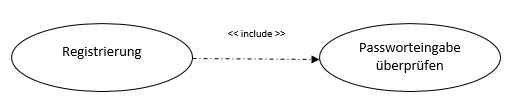
\includegraphics[scale=1]{Include_Use-Case.jpg}
\\
\\
Extend-Beziehung:
\\
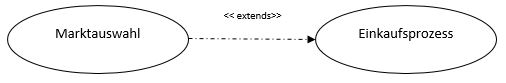
\includegraphics[scale=1]{Extend_Use-Case.jpg}
\\
\newpage
\subsection{Projektorganisation}
%MH: ich weis ja nicht wer von euch welchen teil geschrieben hat, aber ich würde mich inhaltlich gern nochmal über diese Absatz unterhalten
%AK: haben uns ja darüber bereits unterhalten- Änderung am 23.12. vorgenommen
Am 02. Oktober 2015 fand das erste Meeting mit der gesamten Projektgruppe der EinkaufsApp statt, hierbei wurden Absprachen über das weitere Vorgehen und die Projektumsetzung der Ideen und Ziele getroffen.
Das gesamte Team teilte sich zur optimalen Zielerfüllung in die Untergruppen Dokumentation, Design und Entwicklung auf.
Der Projektleiter und in diesem Falle auch Projektmanager wurde ebenso an diesem Tag ernannt.
Als Projektmanager war er nun für die Team- und Projektorganisation zuständig. Dazu gehört unter anderem das Einhalten der Projekt- und Meilensteinplanung und das Erfüllen der Projektziele.
Jegliche Unterhaltung basierte auf Mailverkehr oder fand durch Telefonkonferenzen statt. Jede Untergruppe musste sich selbst organisieren und wöchentlich ein Update dem Projektleiter zukommen lassen. Jeden Montag fanden Status-Telefonkonferenzen statt, wo sich alle Teammitglieder zusammenfanden und über den aktuellen Stand der Untergruppen informierten und über aufgekommene Probleme diskutierten. 
Die Untergruppen einigten sich außerdem auf Tools, die effizient und sinnvoll zur Umsetzung der anstehenden Aktivitäten und zum Einhalten der Projektziele verwendet wurden. 
%AK-Änderung-Ende

\newpage
\subsubsection{Anforderungskatalog}
%MH: wenn die Doku parallel zur Implementation entstanden ist können hier nicht "ziele für das Projekt" definiert werden (das wäre wieder Planungsphase) --> %AK hab es nun geändert und den Satz raus genommen
In dem hier angeführten Kapitel werden konkrete Ziele für das bevorstehende Projekt formuliert, die auf den zuvor aufgeführten Funktionen der Applikation basieren.
Die einzeln genutzten Tools die im Pflichtenheft, welches sich im Anhang befindet, festgehalten sind, werden hier den einzelnen Arbeitsgruppen zugewiesen.
\\
%MH: in dem Bild sollte bei "Umgesetzt von" sollte eher stehen "Entwicklung" oder wahlweise von den "Entwicklern"
%MH: insgesammt bitte nochmal mit mir über die Organisation der Tabelle sprechen! und wenn möglich könnte es geminhin sinvoll sein PDFs einzubinden anstatt von bildern

%way to go for graphics
%negative \hspace um das bild nach links zu verschieben und trim um nicht die ganzen weißen bereiche der pdf zu übernehmen
\hspace*{-10mm} 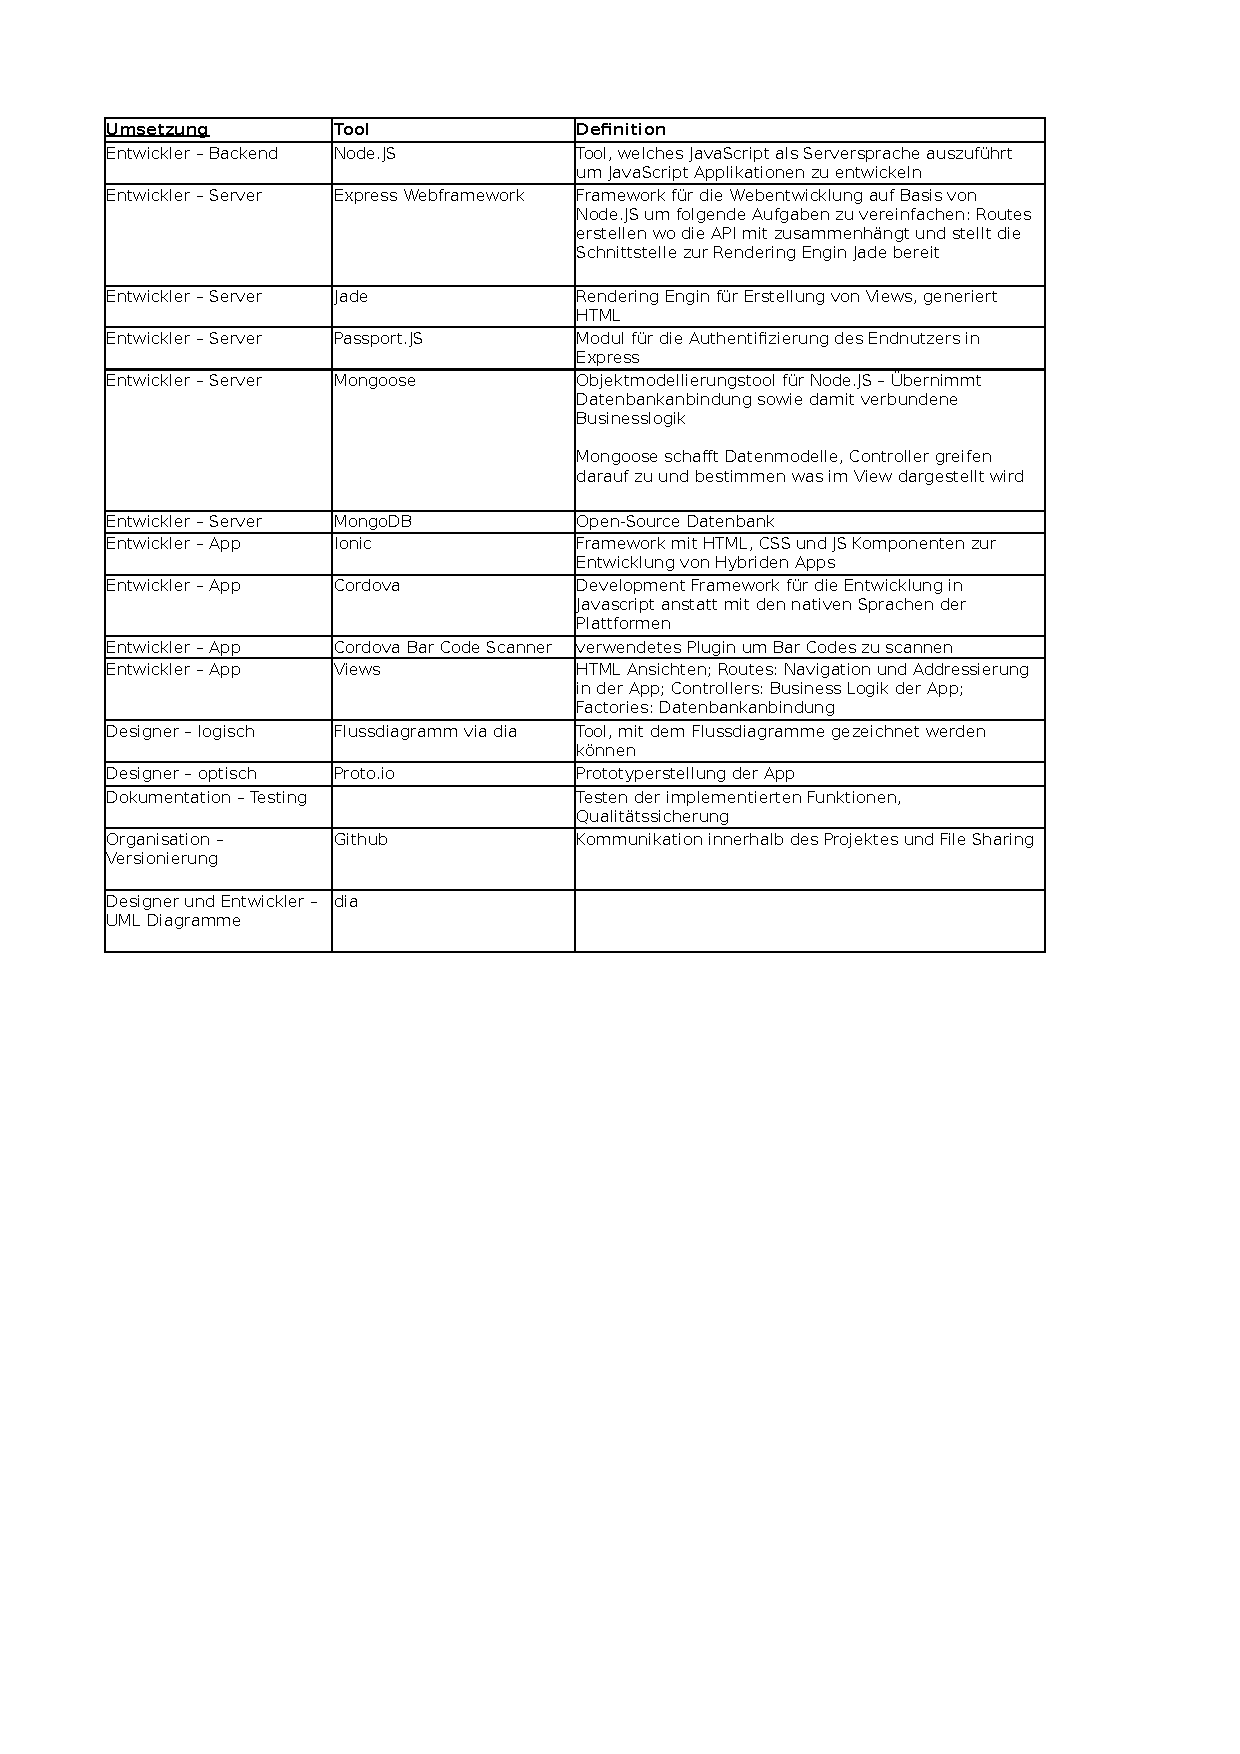
\includegraphics[trim = 17mm 130mm 0mm 20mm]{Anforderungskatalog.pdf}
\\
\footnotesize Tabelle 1: Anforderungsanalyse
\normalsize
\\
\newpage
\subsubsection{Ist-Analyse}
%MH: für eine schlüssige Doku würde hier die Frage aufkommen "warum hab ich das denn vor dem Projekt gemacht???" - außerdem geht es nicht drum mich selbst zu beweiräuchern 
%MH: es sollte mehr in die Richtung gehen "eien Grundanforderung an den Datenbestand ging bereits aus der aufgabe hervor" oder "wurde bereits zu beginn in das Projekt überneommen" - gerne nochmal an mich herantreten
Aus vorangegangener Erfahrung mit dem Thema der automatisierte Unterstützung durch eine App bei Einkäufen im privaten bereich ist ein Grobkonzept, eines ER-Modells, bereits in das Projekt überführt worden. Dieses wurde verwendet, um ein Grundveständnis beim designen und implementieren zu erzeugen. 
\\
\\
\hspace*{-20mm} 
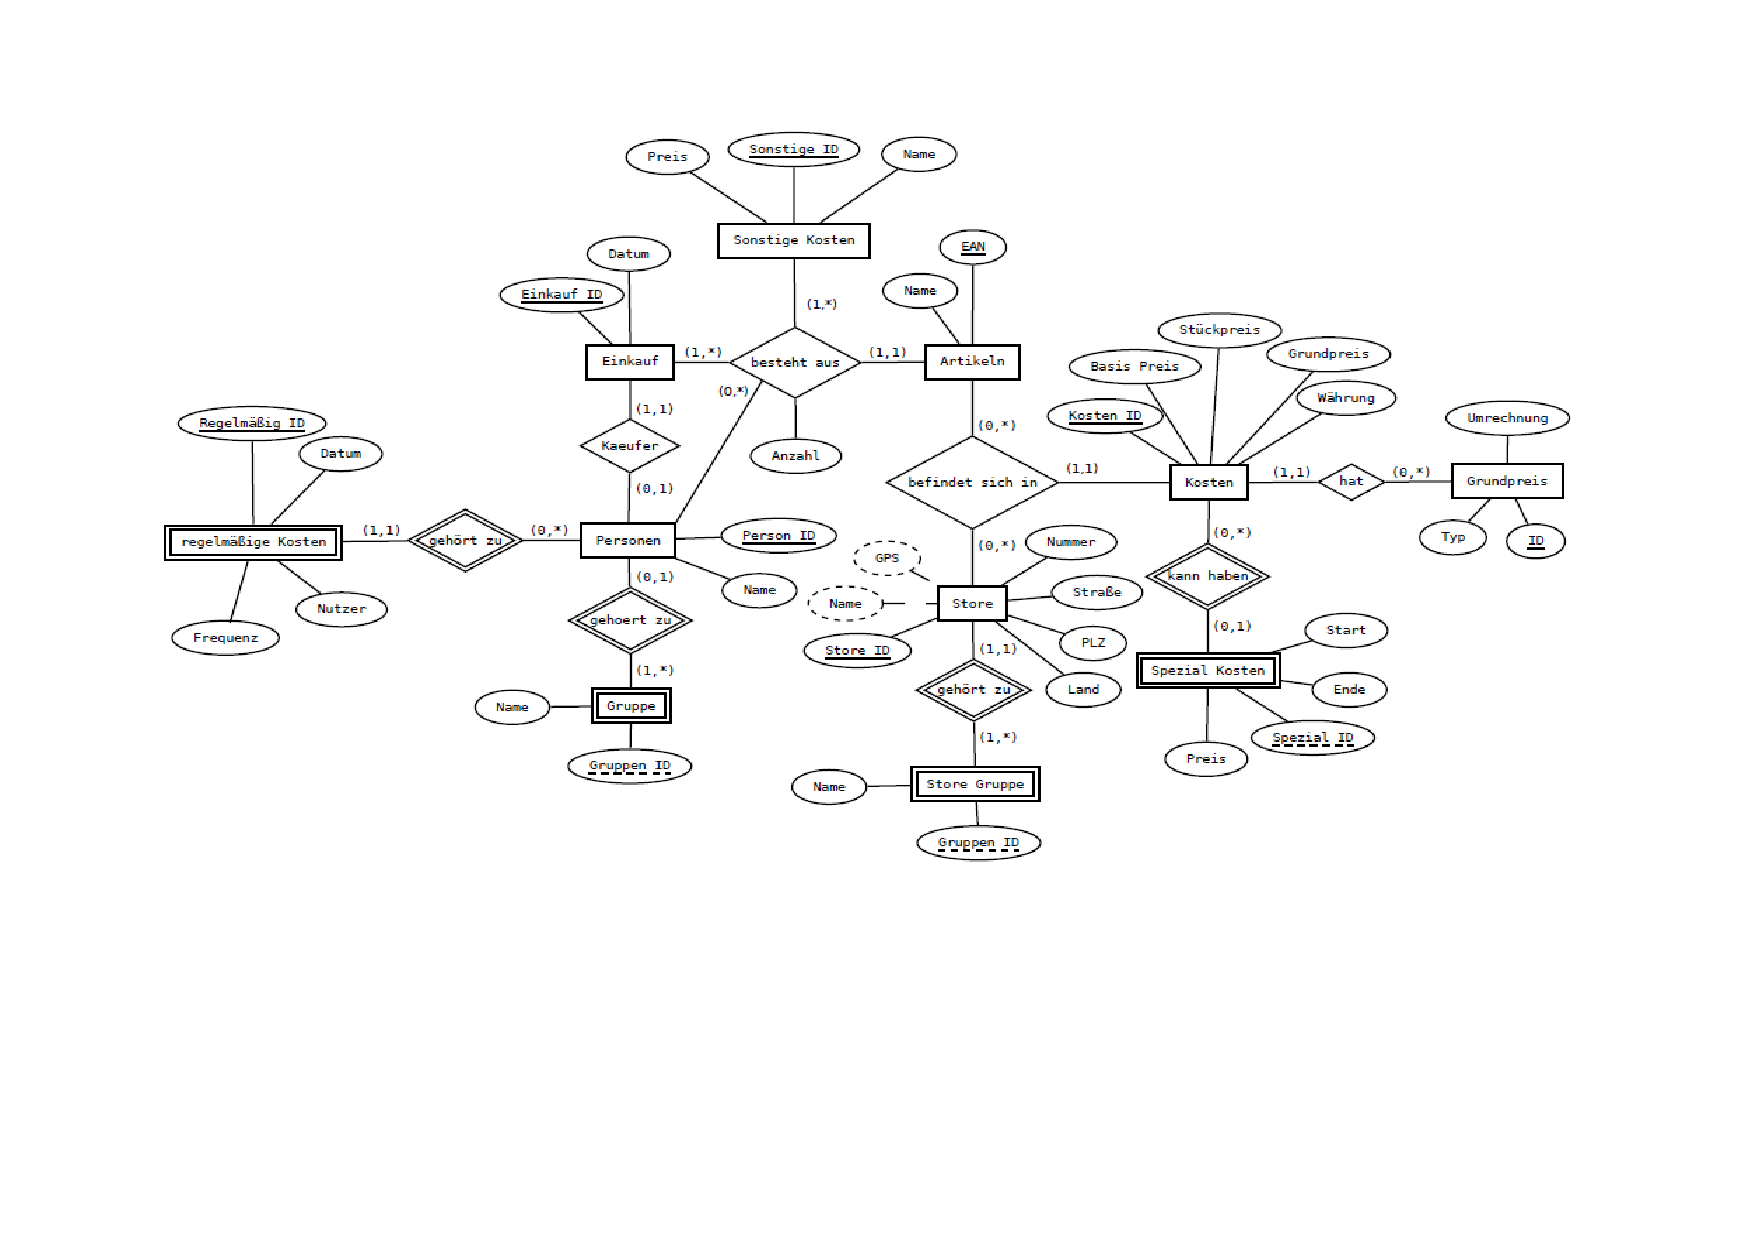
\includegraphics[trim = 15mm 40mm 0mm 20mm, clip, scale=0.7]{ER-Modell.pdf}
\linebreak
\footnotesize Abbildung 2: ER - Modell
\\
\normalsize
\linebreak
\\
Zu Beginn wurden die jeweiligen Kompetenzen der Projektmitarbeiter vor der Durchführung des Projektes aufgenommen. 
Aus diesen leiteten sich die Zugehörigkeiten jeder einzelnen Person in die Projektgruppen Dokumentation, Entwicklung und Design ab. 
\\
\\
\hspace*{-10mm} 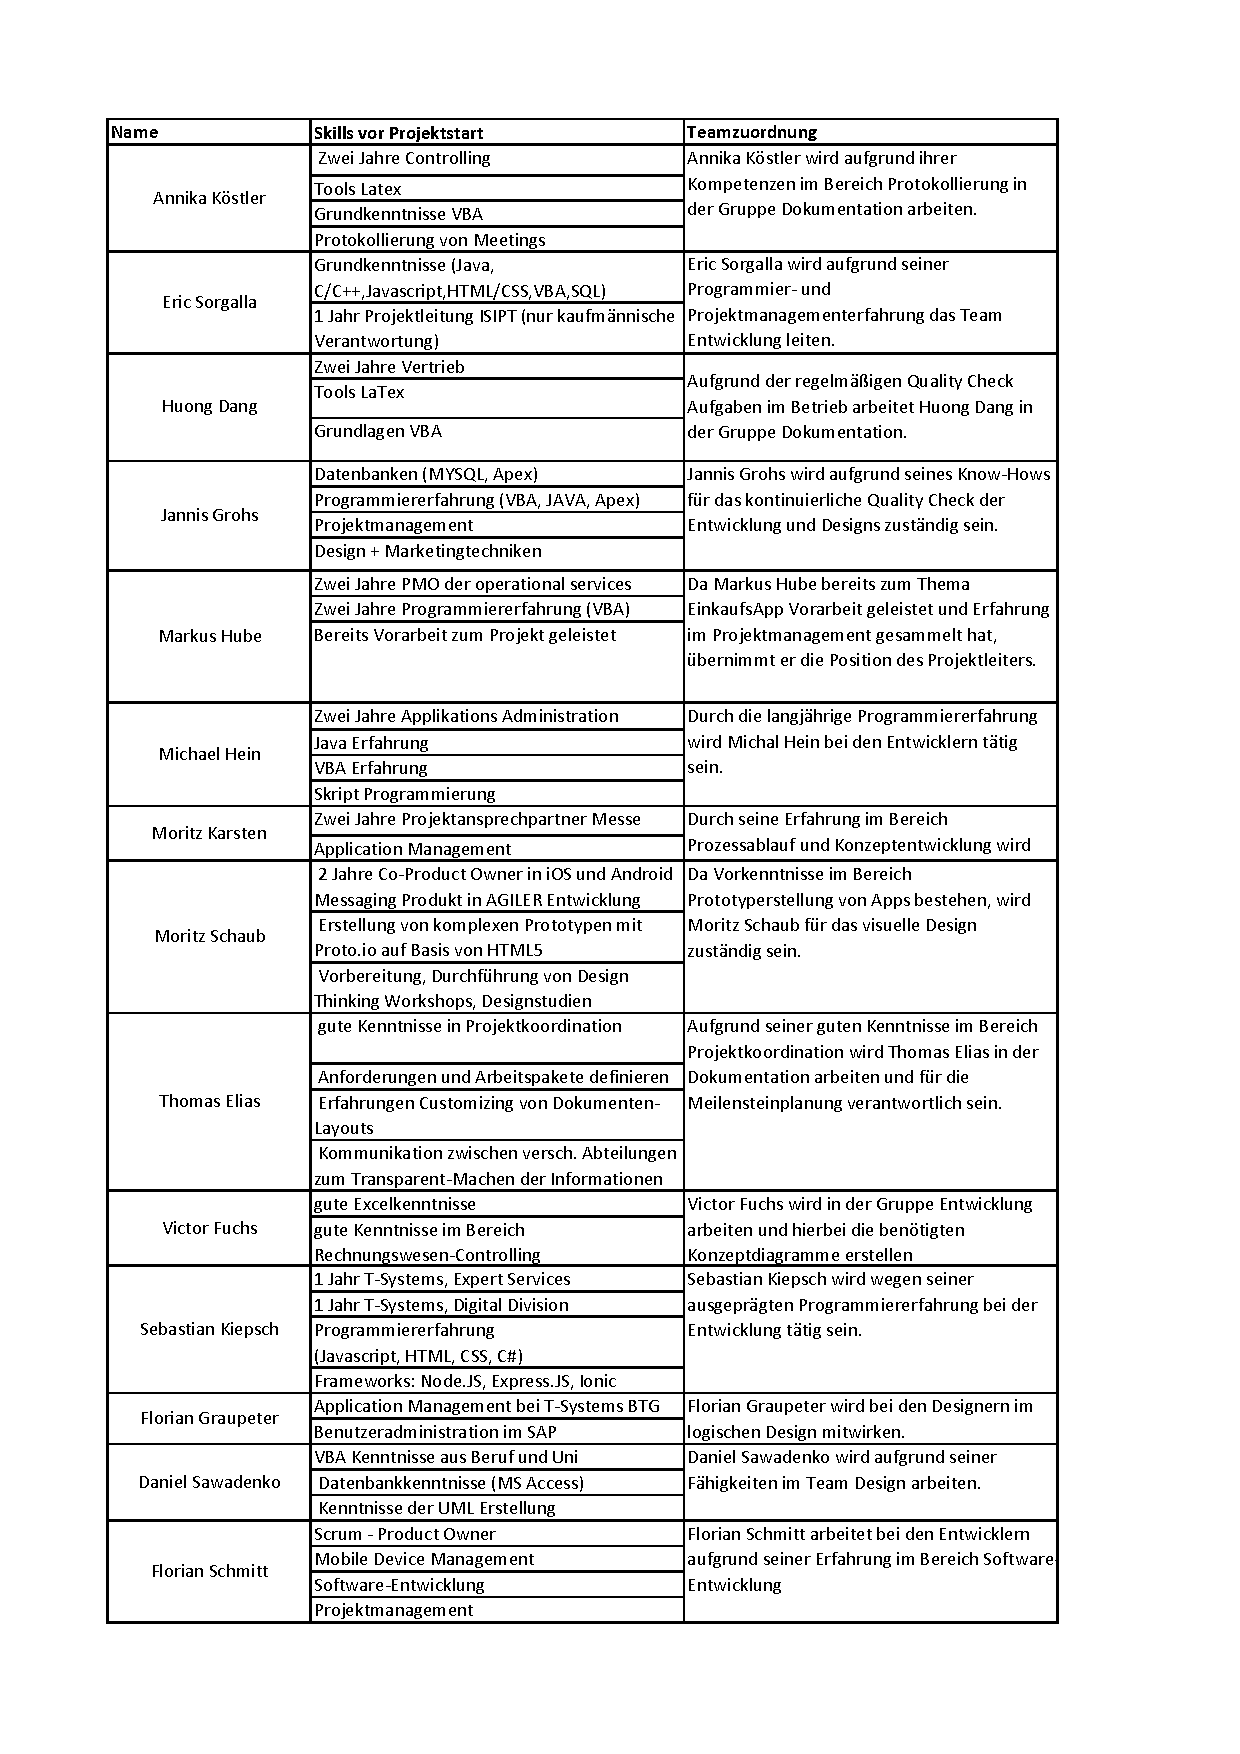
\includegraphics[trim = 15mm 0mm 0mm 20mm,clip,scale=0.8]{Skillliste.pdf}
\footnotesize Tabelle 2: Ist-Analyse
\\
\normalsize
\linebreak
\\
%TO DO - darstellen durch eine eingebundene PDF
%\begin{longtable}{|m{5cm}|m{5cm}|m{5cm}|}
%\hline
%\textbf {Name} & \textbf {Skills} & \textbf {Teamzuordnung} \\
%\hline
%\centering Annika Köstler & \begin {itemize}
%\item Zwei Jahre Arbeit im Controlling
%\item Tools:LaTex
%\item Grundkenntnisse VBA
%\item Protokollierung von Meetings
%\end{itemize}
%& Annika Köstler wird aufgrund ihrer Kompetenzen im Bereich Protokollierung in der Gruppe Dokumentation arbeiten.
%\\
%\hline
%\centering Eric Sorgalla & 
%\begin {itemize}
%\item Grundkenntnisse (Java, C/C++, Javascript, HTML/CSS, VBA, SQL)
%\item 1 Jahr Projektleitung ISIPT (nur kaufmännische Verantwortung) 
%\end {itemize}
%& Eric Sorgalla wird aufgrund seiner Programmiererfahrung bei den Entwicklern arbeiten
%
%\\
%\hline
%\centering Huong Dang & \begin {itemize}
%\item Zwei Jahre Vertrieb
%\item Tools LaTex
%\item Grundlagen VBA 
%\end {itemize}
%& Aufgrund der regelmäßigen Quality Check Aufgaben im Betrieb arbeitet Huong Dang in der Gruppe Dokumentation.
%
%\\
%\hline
%\centering Jannis Grohs & \begin {itemize}
%\item Datenbanken (MYSQL, Apex)
%\item Programmiererfahrung (VBA, JAVA, Apex)
%\item Projektmanagement 
%\item Design - und Marketingtechniken
%\end {itemize}
%& Jannis Grohs wird aufgrund seines Know-Hows für das kontinuierliche Quality Check der Entwicklung und Designs zuständig sein.
%
%\\
%\hline
%\centering Markus Hube & \begin {itemize}
%\item Zwei Jahre PMO der operational services
%\item Zwei Jahre Programmiererfahrung (VBA)
%\item Bereits Vorarbeit zum Thema EinkaufsApp geleistet 
%\end {itemize}
%& Da Markus Hube bereits zum Thema EinkaufsApp Vorarbeit geleistet und Erfahrung im Projektmanagement gesammelt hat, übernimmt er die Position des Projektleiters.
%
%\\
%\hline
%\centering Michael Hein & \begin {itemize}
%\item Zwei Jahre Applikations Administration
%\item Java Erfahrung
%\item VBA Erfahrung
%\item Skript Programmierung
%\end {itemize}
%& Durch Michael Heins langjähriger Programmiererfahrung wird er bei den Entwicklern tätig sein.
%
%\\
%\hline
%\centering Moritz Karsten & \begin {itemize}
%\item  Zwei Jahre Projektansprechpartner Messe Berlin
%\item  Application Management
%\end {itemize}
%& Durch seine Erfahrung im Bereich Prozessablauf und Konzeptentwicklung wird Moritz Karsten bei der Gruppe Design arbeiten.
%\\
%\hline
%\centering Moritz Schaub & \begin {itemize}
%\item  Zwei Jahre Co-Product Owner in iOS und Android Messaging Produkt in AGILER Entwicklung (internationales, crossfunktionales Team)
%\item  Erstellung von komplexen Prototypen mit Proto.io auf Basis von HTML5
%\item Durchführung von Design Thinking Workshops
%\end {itemize}
%& Da Moritz Schaub Vorkenntnisse im Bereich Prototyperstellung von Apps hat, wird er für das visuelle Design zuständig sein.
%
%\\
%\hline
%\centering Thomas Elias & \begin {itemize}
%\item gute Kenntnisse in Projektkoordination
%\item Anforderungen und Arbeitspakete definieren
%\item Erfahrungen Customizing von Dokumenten-Layouts
%\item Kommunikation zwischen versch. Abteilungen zum Transparent-Machen der Informationen
%\end {itemize}
%& Aufgrund seiner guten Kenntnisse im Bereich Projektkoordination wird Thomas Elias in der Dokumentation arbeiten und für die Meilensteinplanung verantwortlich sein.
%
%\\
%\hline
%\centering Victor Fuchs & \begin {itemize}
%\item  gute Excelkenntnisse
%\item  gute Kenntnisse im Rechnungswesen und Controlling
%\end {itemize}
%& Victor Fuchs wird in der Gruppe Entwicklung arbeiten und hierbei die benötigten Konzeptdiagramme erstellen.
%\\
%\end{longtable}
\newline
\newline
Insgesamt gibt es demnach drei Designer, fünf Entwickler und drei Dokumentatoren, die parallel den stetigen Quality Check durchführen.
\\
\subsubsection{Arbeitsplanung}
Zu Beginn der Projektorganisation wurde von der Dokumentation ein grober Plan erstellt, der eine Einteilung der Teams in organisatorische Einheiten aufzeigt und einen Rahmen für die Planung der Aufgaben, beziehungsweise Arbeitspakete, vorgibt. 
Es wurde ein organisatorisches Grundgerüst geschaffen, das allen Gruppen als Orientierung dient und gleichzeitig zur eigenständigen Organisation, sowie Bearbeitung der Arbeitspakete motiviert:
\\
\\
%MH: hier taucht wieder die Planungsphase auf...
\hspace*{-10mm} 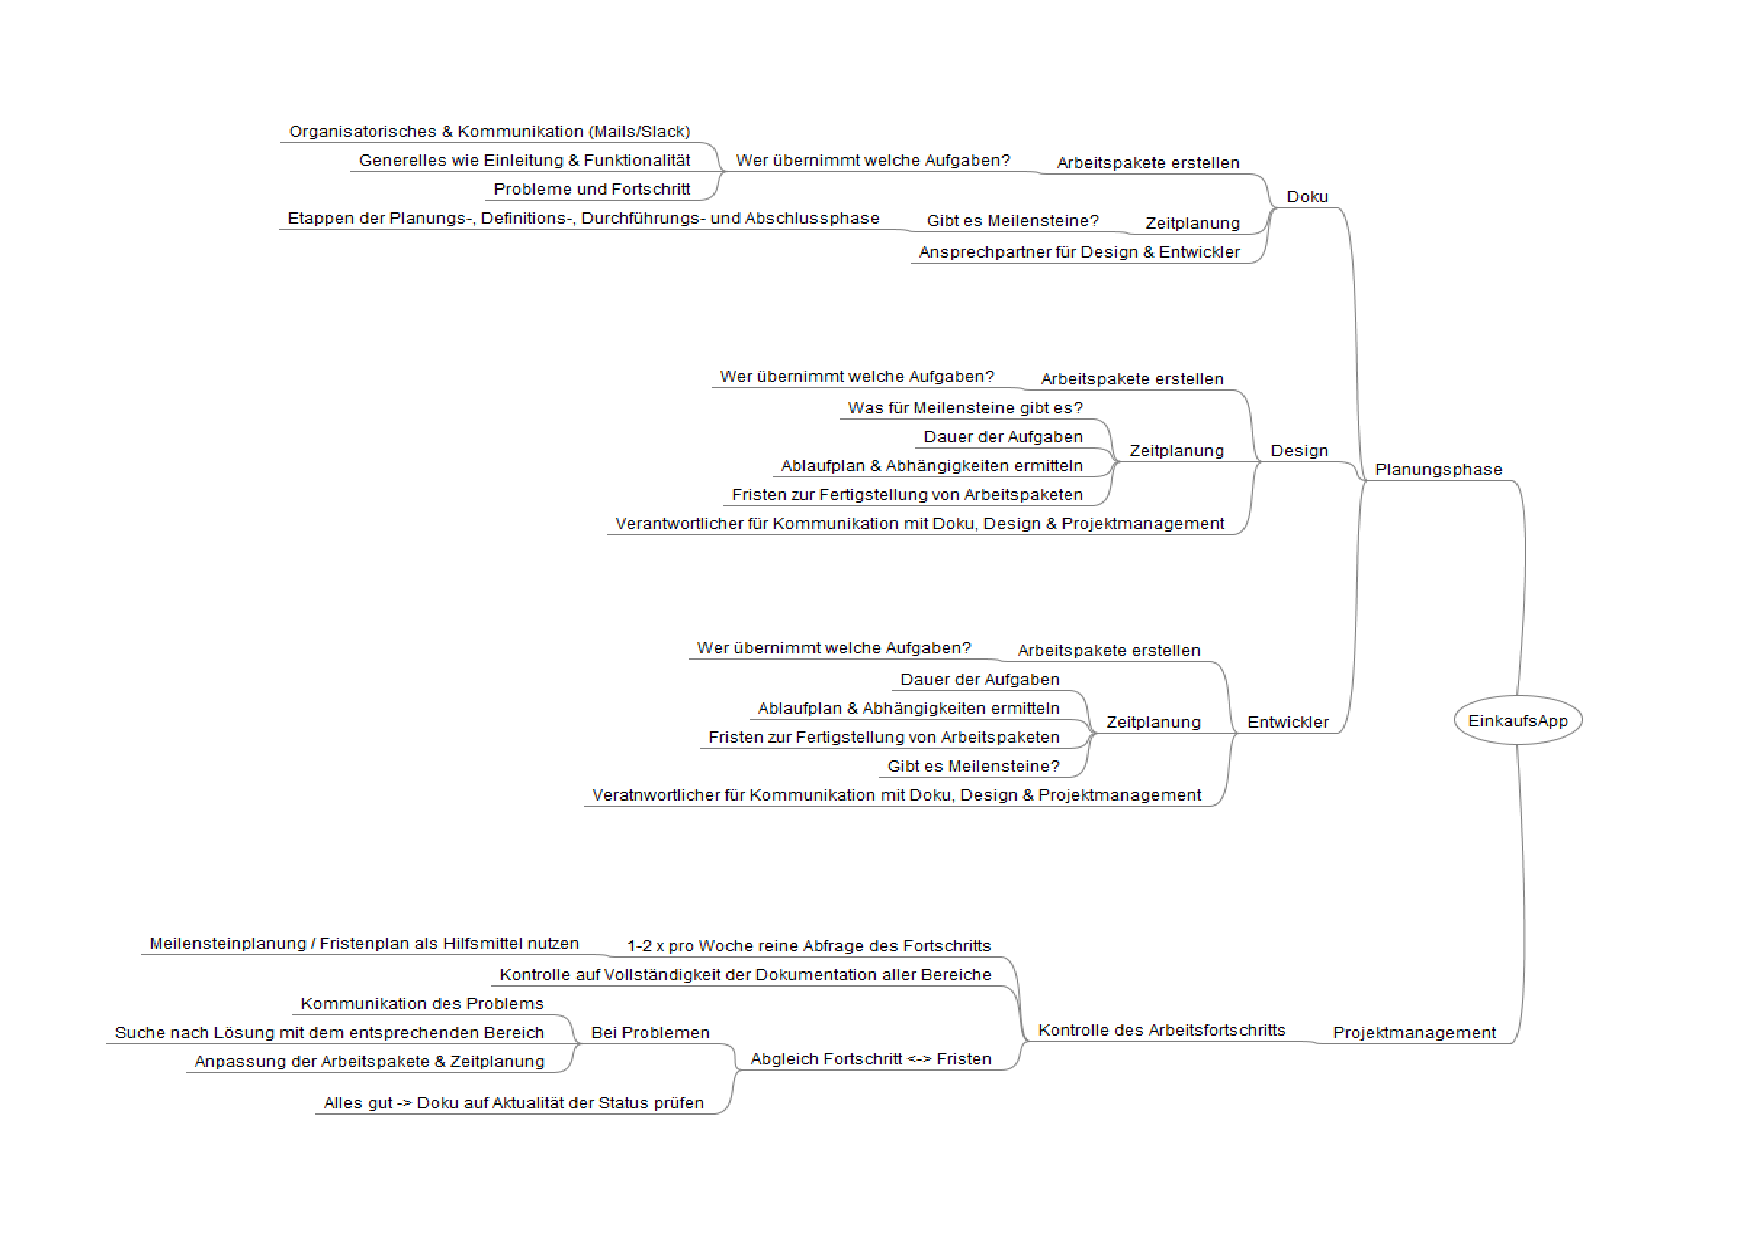
\includegraphics[trim = 20mm 0mm 0mm 20mm,clip,scale=0.7]{Aktivitaetsliste.pdf}
\\
\footnotesize Abbildung 1: Aktivitätsliste
\normalsize
\\
\linebreak
\subsubsection*{Meilensteinplanung}
\hspace*{-10mm} 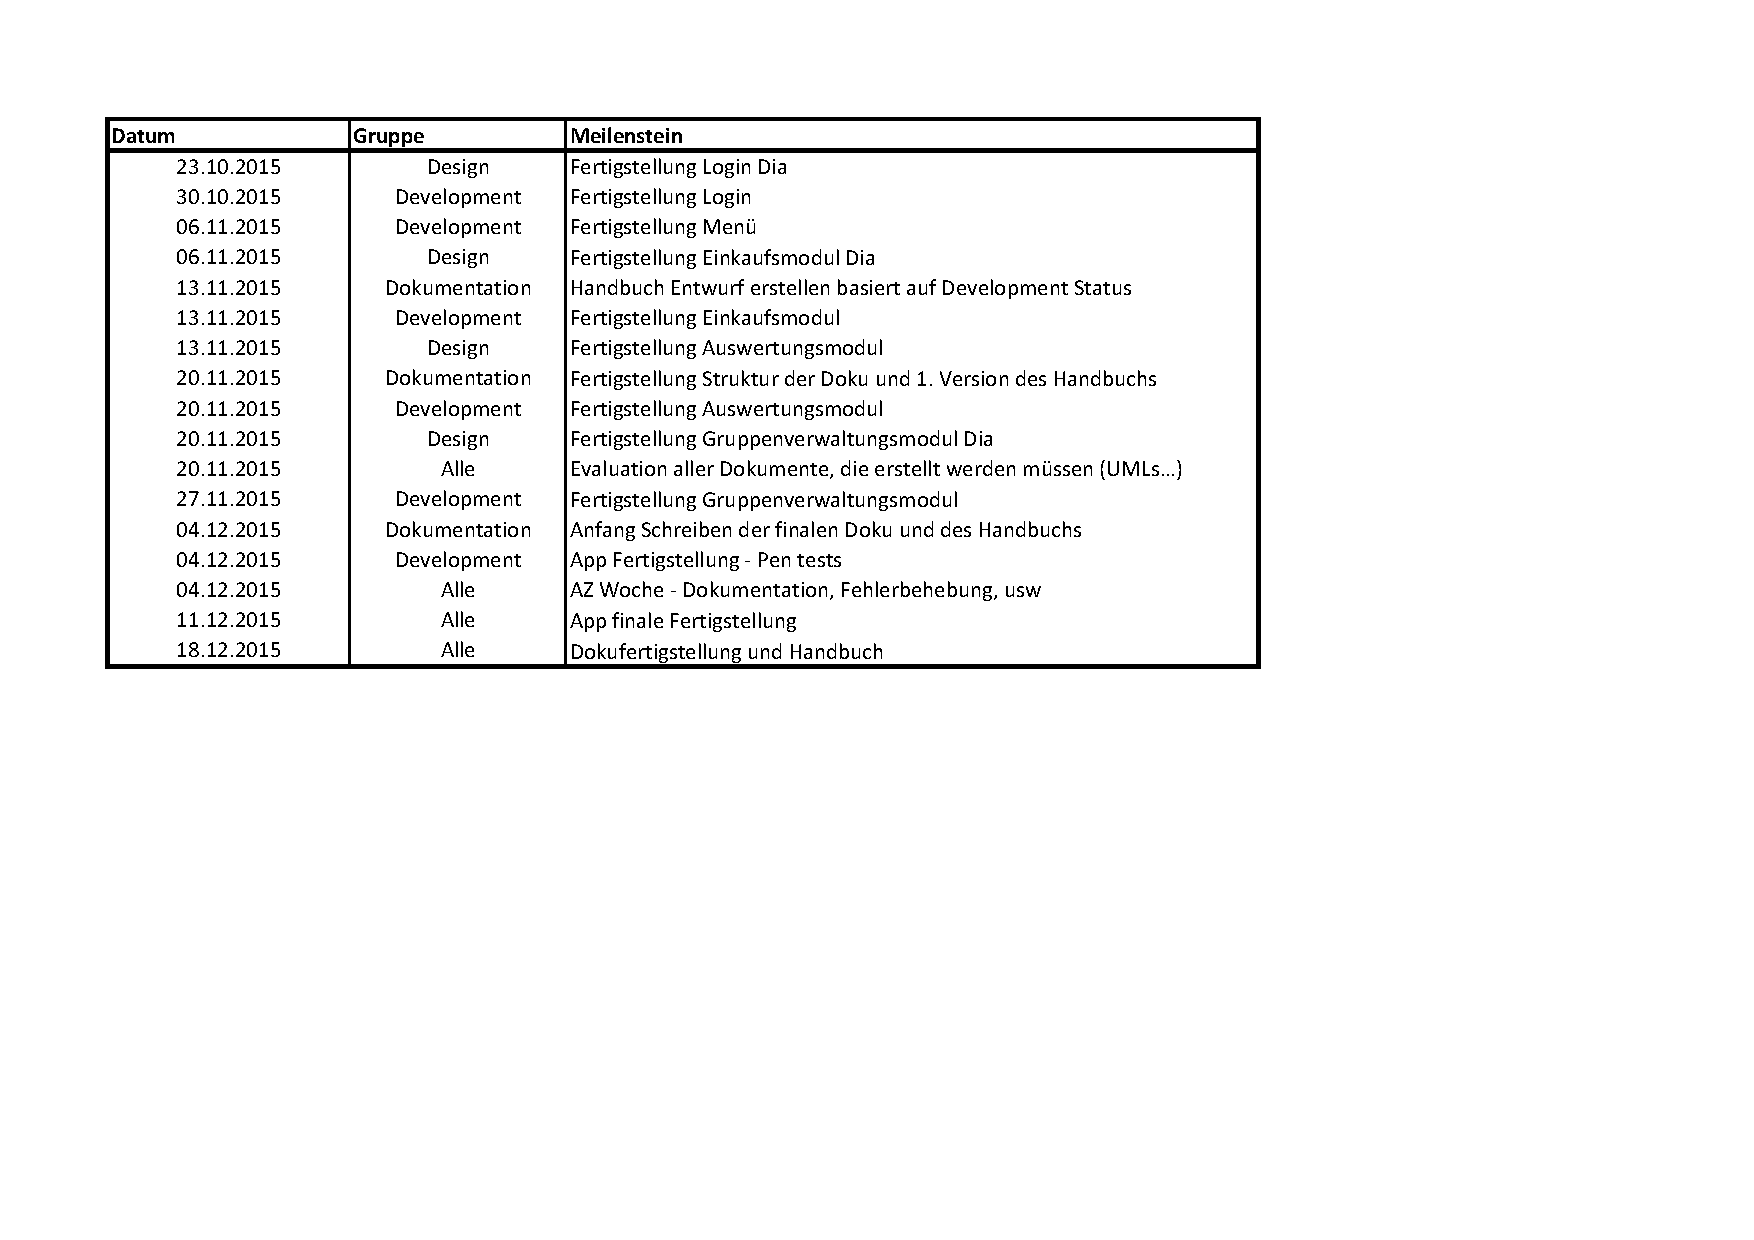
\includegraphics[trim = 10mm 90mm 10mm 20mm,clip, scale=0.9]{Meilensteine.pdf}
\\
%MH: holt euch ganz schnell nochmal fixierte Aussagen dazu von Eric, wenn er euch dazu überhaupt etwas sagen kann. Wenn nicht komplett anders darstellen oder rausnehmen.
\footnotesize Abbildung 2: Meilensteine
\normalsize

\subsubsection{Agiles Projektmanagement}
%MH: ganz dringend inhaltlich nochmal mit mir besprechen!!!
Nachdem ein grober organisatorischer Rahmen für das Projekt von der Gruppe Dokumentation vorgegeben wurde, haben die einzelnen Gruppen, durch agile Projektmanagement-Methoden,  ihre Arbeitspakete und Ablaufpläne festgelegt. 
Die Dokumentation erstellte Arbeitspakete für alle Gruppen und jedes Projektmitglied hat sich nach dem Pull-Prinzip – bekannt aus der Projektmanagement-Methode Kanban – seine Arbeitspakete abgeholt und eine Bearbeitungsfrist definiert. 
In der Gruppe der Entwickler wurde unter Zuhilfenahme des Tools „Trello“ die Planung und Durchführung der Arbeitspakete definiert. Trello ist ein Web-Dienst, der ein Board anbietet, um Arbeitspakete gemäß agiler Projektmanagement-Methoden zu bearbeiten und Arbeitsfortschritte transparent darzustellen. 
Die Designer haben ihre Arbeitspakete auf Basis eines Ablaufplanes verteilt. Es wurden die Phasen Prototyp-Entwurf, Prototyp-Review, Prototyp-Modifikationen und Prototyp-Test und Prototyp-Abnahme durchlaufen.
\newpage
\subsection{Sicherheit}
Sobald Daten eines Nutzers für eine Applikation gespeichert werden, wird ein gewisser Standard an Sicherheit gefordert, damit keinen Dritten diese Daten zugänglich werden.
In der EinkaufsApp wurden folgende Maßnahmen getroffen um dies gewährleisten zu können:
\\
1. Der Nutzer startet durch die Eingabe von Benutzername und persönlichem Password eine Session, die Ihn bei jeder Anfrage an den Server authentifiziert.
\\
2. Alle Passwörter werden als Einweg-Hash in der Datenbank gespeichert. Bei der Anmeldung wird das Passwort dem gleichen Verfahren unterzogen und dann die resultiereden Zeichenfolge mit der, in der Datenbank gespeicherten, abgeglichen.
\\ 
%MH: was ist der Inhalt dieser Aussage?
%2. In Verbindung mit dem Nutzernamen wird sichergestellt, dass es sich auch um den richtigen Nutzer handelt.
\\
3. Die Verwendung des SSL-Protokolls (Secure Socket Layer) sorgt für  den Aufbau eines geschützten Kanals vor der eigentlichen HTTP-Kommunikation, so dass die Nutzerdaten für Dritte nicht zugängig sind. 
Dies bedeutet: Die Nutzerdaten werden in einem standart Web-Formular eingetragen (Login-Screen) und mittels POST-Request an den Server gesendet. 
Da der TCP-Kanal verschlüsselt ist, haben Dritte keinen Zugriff auf die vom Nutzer eingegebenen Daten innerhalb des POST-Requests, was wiederum die gesicherte Übertragung von Nutzernamen und Passwort bewirkt.

\newpage
\section{Durchführungsphase}
\subsection*{Architektur}

%TO DO - MH: bisschen architetktur aufschreiben

In diesem Abschnitt wird die Funktionsweise der EinkaufsApp beschrieben. Dabei werden die einzelnen Hauptprozesse separat vorgestellt und deren technische Umsetzung erläutert. Die Hauptprozesse sind unterteilt in den Login und die Registrierung des Nutzers, den Einkaufsprozess, die Nutzerverwaltung und die Auswertung. 
%HD - 23.12.2015: willst du den unteren Text mit reinnehmen?
%Generell wurde in der Entwicklung nach dem Modell-View-Controller Prinzip gearbeitet. Nachdem die Prozesslogik der Designer stand („Modell“), wurden die einzelnen Views, also die visuelle Darstellung der zu implementierten Funktion, die der Nutzer am Ende sieht, entwickelt und welche schlussendlich über die „Controller“ mit der Logik versehen wurden. Jedes einzelne View hat dabei seinen eigenen Route.

\subsection*{Einleitung}
Die genannten Hauptprozesse stehen, wie in dem folgenden Diagramm zu sehen ist, in Relation. Dabei wurden die Views als einzelne Klassen dargestellt:
\\
\\
%MH: ist dem Leser an der stelle Klar was "Views" sind???
\hspace*{-10mm} 
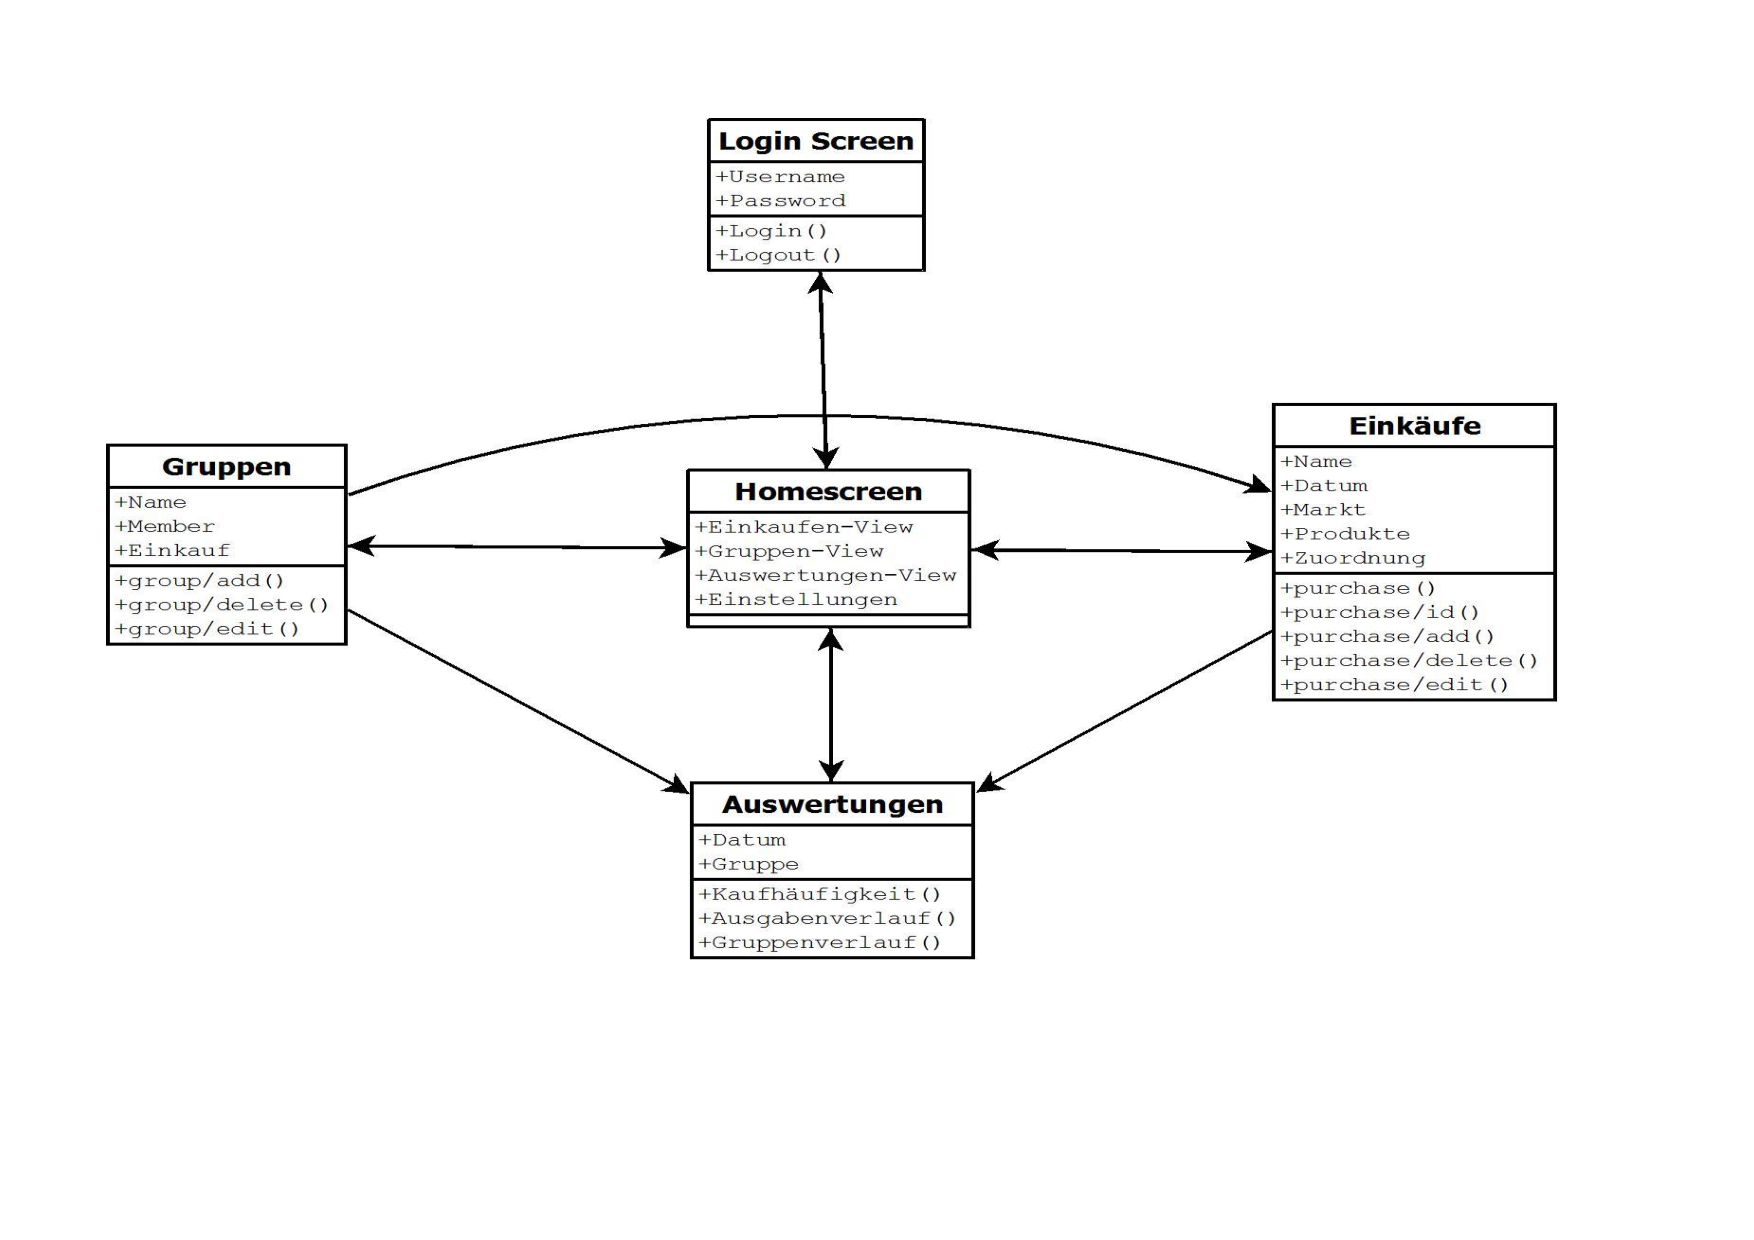
\includegraphics[trim = 17mm 30mm 0mm 20mm,clip,scale=0.7]{Klassendiagramm.pdf}
\\
\footnotesize Abbildung 3: Klassendiagramm
\normalsize

\subsection{Registrierung}
Um die EinkaufsApp zu nutzen, muss sich jeder Nutzer mittels einer Email-Adresse und einem Kennwort für der App registrieren.
Eine Registrierung ist bei dieser App unentbehrlich, da für jeden Nutzer ein Profil angelegt wird und diesem Profil innerhalb der Datenbenk die Produkte und Finanzen zugeordnet werden.
In den folgenden Unterpunkten wird der Prozess der Registrierung jeweils von den Designern und Entwicklern beschrieben.
\subsubsection*{Design}
Die Designer haben zu der Registrierung und zu dem Login, welcher im Punkt 3.4 behandelt wird, das folgende Flussdiagramm entworfen:
\\
\hspace*{-10mm} 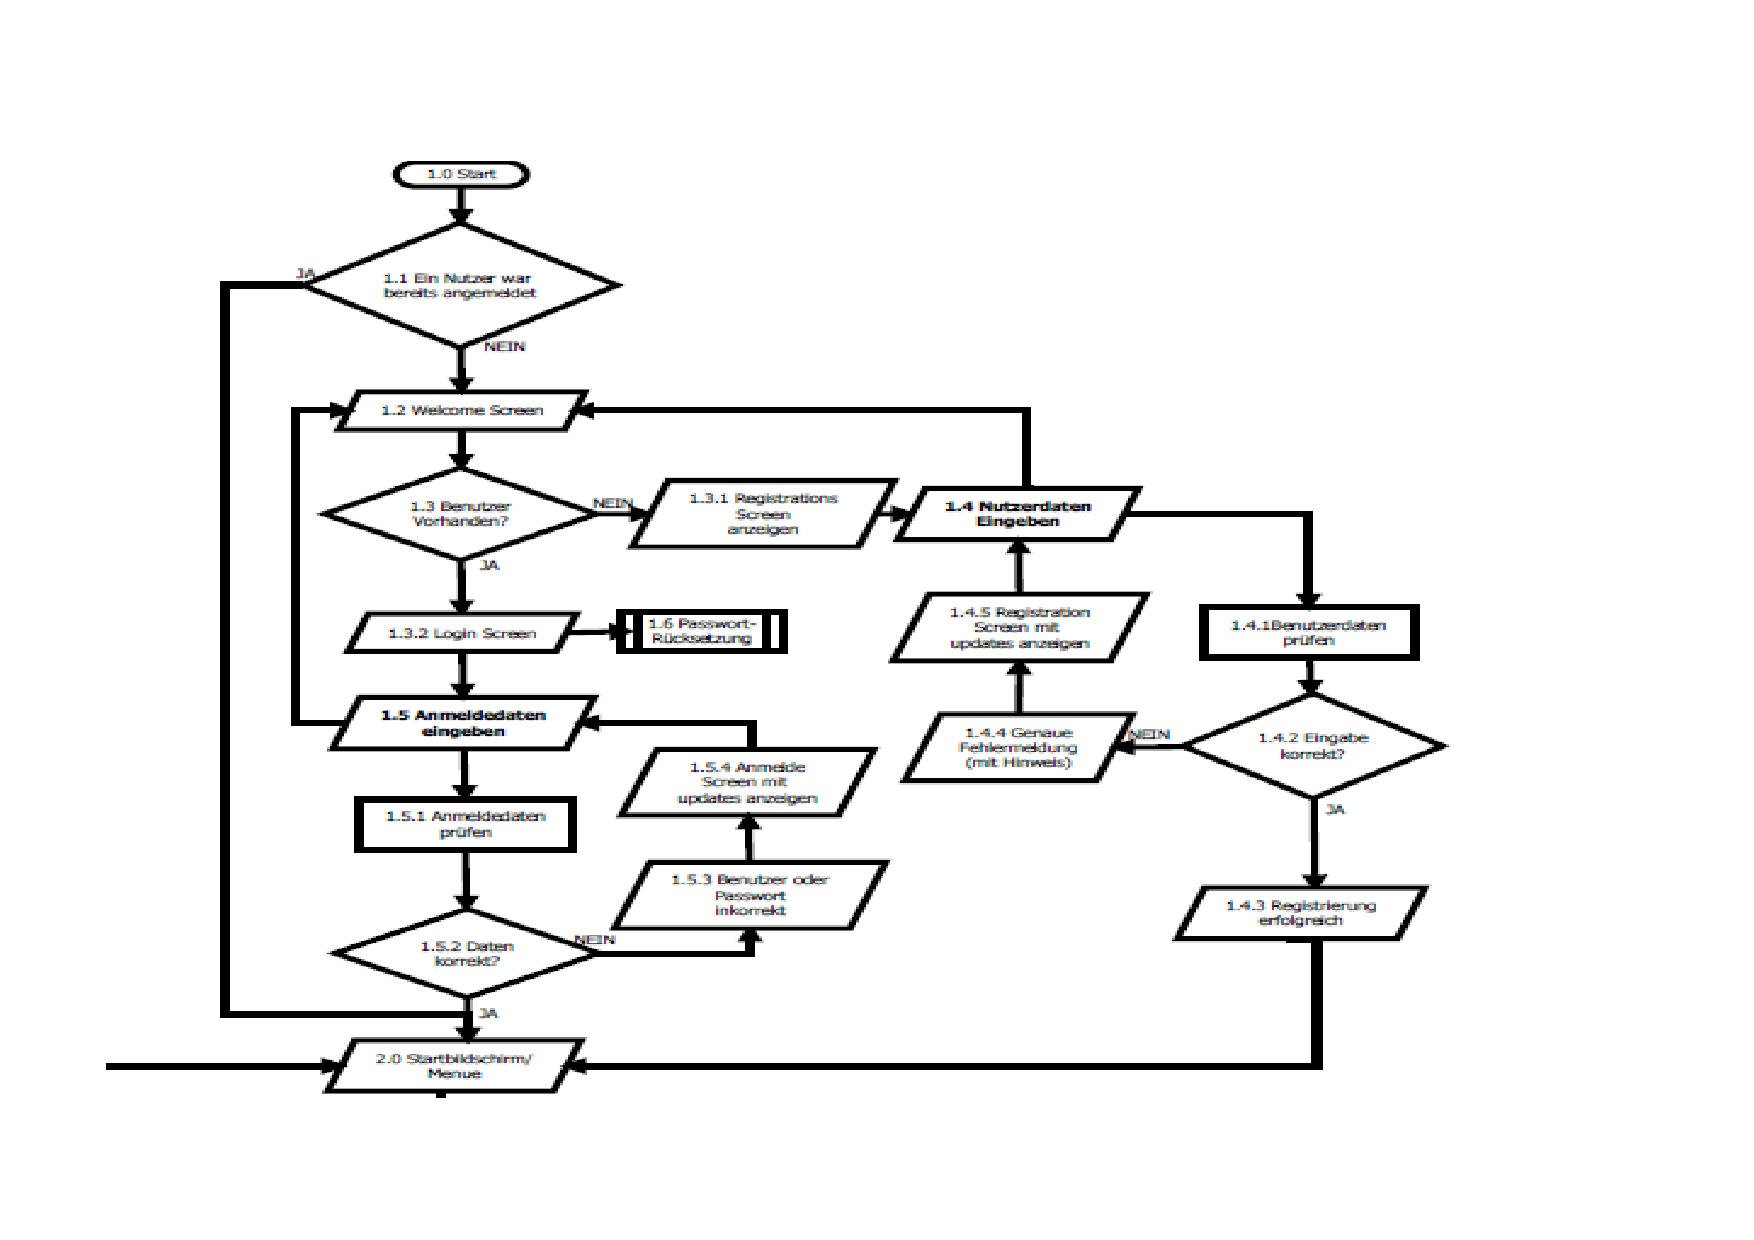
\includegraphics[trim = 17mm 0mm 0mm 20mm, clip, scale=0.8]{Login-PDF.pdf}
\footnotesize Abbildung 4: Flussdiagramm Login
\normalsize
\\
\linebreak
Das Flussdiagramm beschreibt sukzessiv den Ablauf des Registrierungs- und des Loginvorgangs, welcher von den Entwicklern daraufhin technisch umgesetzt wurde.
\newpage
\subsubsection*{Entwicklung}
Die Entwickler befassen sich mit den Funktionen der Applikation  und sorgen bei der Registrierung dafür, dass alle Daten ordnungsgemäß geprüft und in die Datenbank eingepflegt werden.
Als Datenbank wird für die App MongoDB genutzt, welche via RoboMongo gemanagt wird. Als Programmiersprache JavaScript.\footnote{Genaueres zu der Datenstruktur können Sie dem angehängten Pflichtenheft entnehmen.} verwendet.

Bei der Registrierung werden die einzelnen Benutzereingaben durch bestimmte Regeln in hinblick auf Länge, Email-Format, Eindeutigkeit, sowie Sicherheitskriterien bei der Passwortvergabe in der Applikation geprüft.\footnote{Die konkreten Regeln der Benutzereingaben können Sie in dem angehängten Handbuch entnehmen.}

Wenn alle Prüfungen erfolgreich waren, wird der Benutzer angelegt und das Passwort verschlüsselt in Form eines Hashs in der Datenbank gespeichert.
\newpage
\subsection{Login}
\subsubsection*{Design}
Das Flussdiagramm der Designer für den Login ist im Abschnitt 3.3 Registrierung zu finden. 
\subsubsection*{Entwicklung}
Die Entwicklung beschäftigt sich mit der Funktionsweise des Logins und prüft hierbei, ob der Benutzer in der Datenbank existiert. Falls dies der Fall ist, wird das Passwort geprüft und bei korrekter Eingabe ist der Login erfolgreich durchgeführt.
Wenn der Benutzer sein Passwort vergessen hat, kann er dieses zurücksetzen lassen. Hierbei bekommt er eine E-Mail an die im Userprofil hinterlegte E-Mail Adresse. Diese Funktionalität ist bereits implementiert, wird aber auf Grund der Sicherheitsbestimmungen der Testumgebung geblockt. Diese enthält ein Token womit es einen Benutzer ermöglicht wird sein Passwort zu ändern. Dieses Token ist genau eine Stunde gültig, danach verfällt es. 
In dem dann aufgerufenen Bilschirm muss der Nutzer nun sein Passwort zweimal eintragen. Daraufhin ändert die Datenbank das Kennwort des Nutzer und speichert dieses.
\newpage
\subsection{Marktauswahl}
Bevor der Einkaufsprozess beginnt muss der Nutzer einen Markt auswählen, hierfür wird der Standort des Nutzers ermittelt via GPS ermittelt und bereits registrierte Märkte in seiner Nähe angezeigt. 
\subsubsection*{Design}
Die Designer haben hierzu, ebenso wie bei der Registrierung und dem Login ein Flussdiagramm erstelt: 
\\
\\
\hspace*{-10mm} 
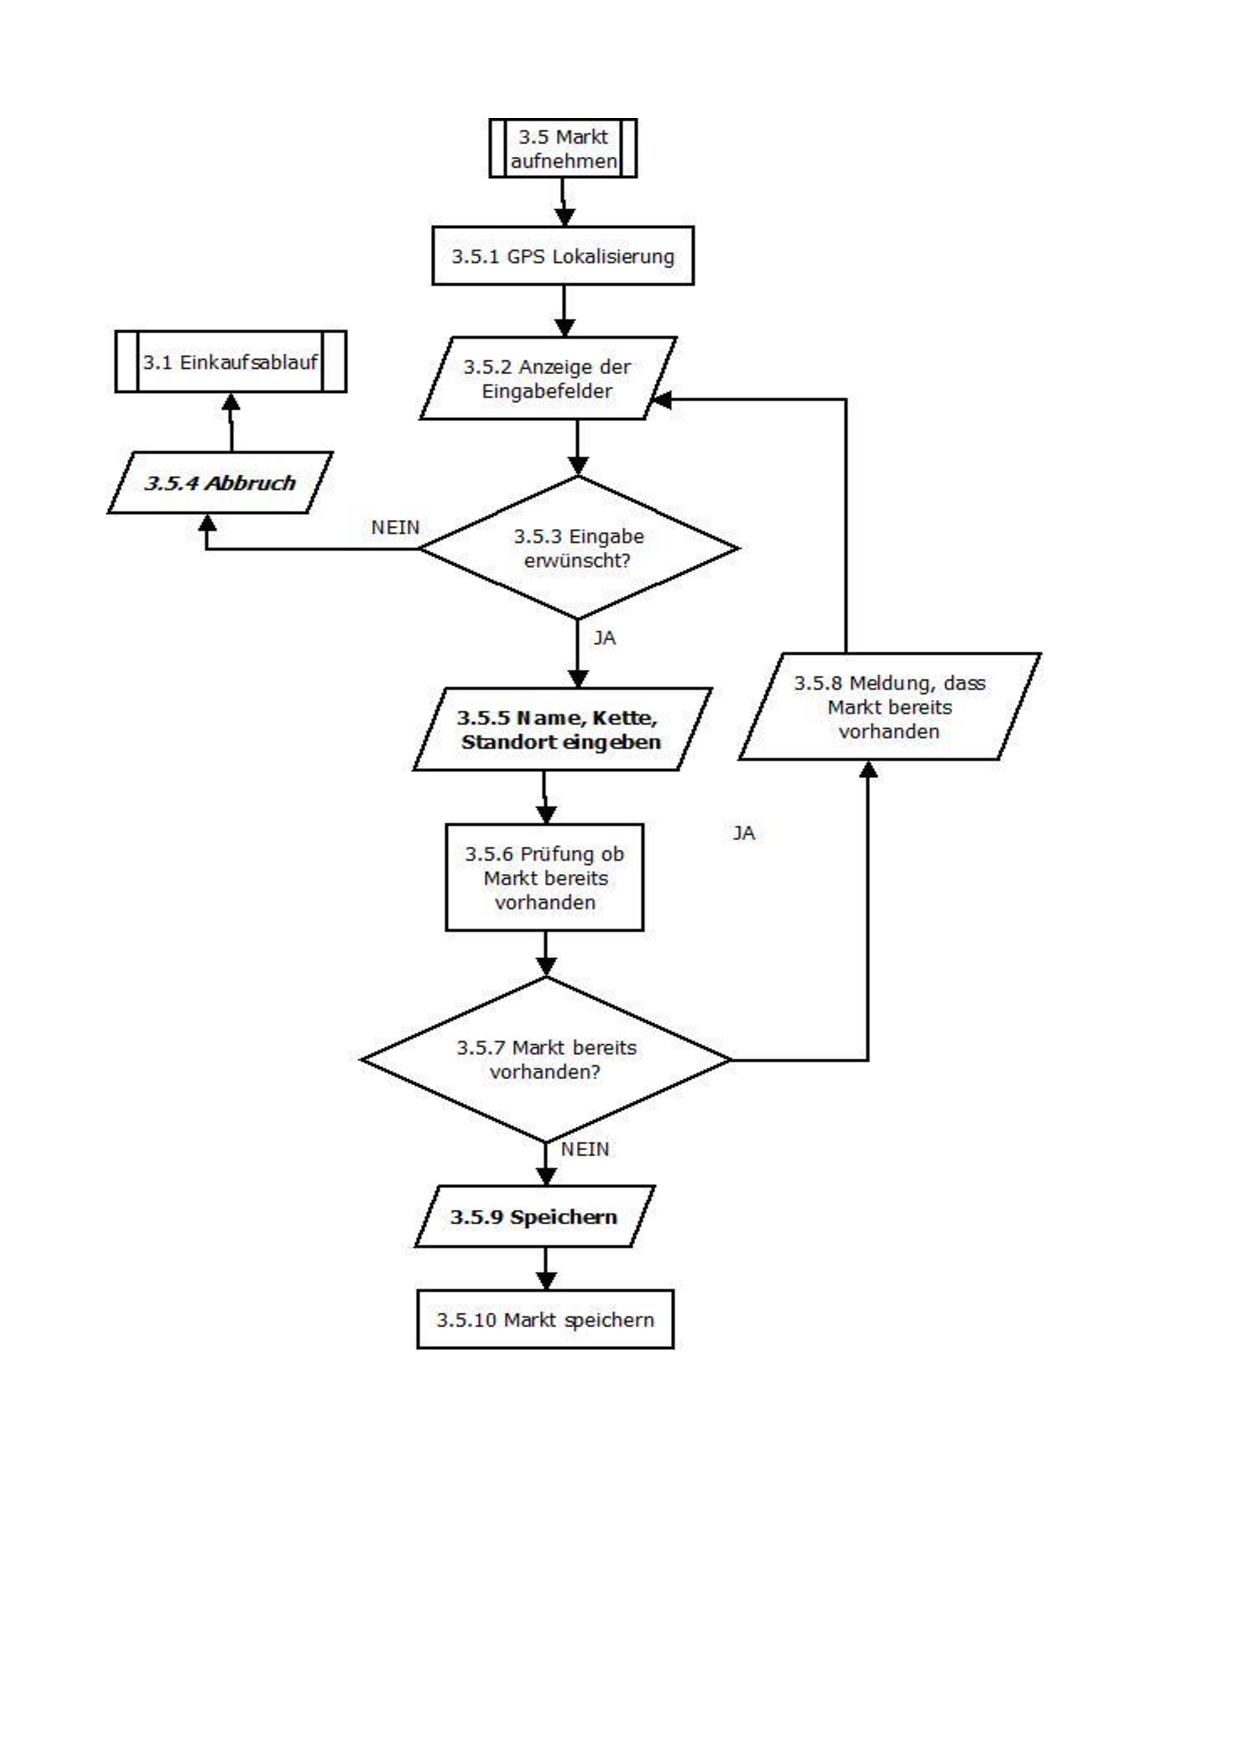
\includegraphics[trim = 17mm 40mm 0mm 20mm, clip, scale=0.9]{Markt-Aufnahme.pdf}
\\
\footnotesize Abbildung 5: Markt-Auswahl
\normalsize
\subsubsection*{Entwicklung}
%TO DO - HD: noch machen^^
%HD - 22.12.2015: Wo kieg ich die Infos her?
%HD - 23.12.2015: Entwicklertext
Der vom Design erstellte Ablauf der Marktauswahl wird direkt in den Einkaufsprozess mit eingebunden. Sobald der Nutzer die Option „Einkaufen“ wählt gelangt dieser in den Marktauswahl-View. Anders als im geplanten Ablauf der Designer, kann der Nutzer selber entscheiden, in welchem Markt er sich gerade befindet, indem er entweder in der direkt aufgeführten Marktliste einen auswählt, oder die Option „Markt hinzufügen“ nutzt. Dies hat technische Gründe, da zurzeit eine Lokalisierung der Märkte via GPS aus Zeitgründen noch nicht umgesetzt wurde.
\newpage
\subsection{Einkaufsverwaltung}
\subsubsection{Design}
Aktivitätsdiagramm „Einkauf einlesen“ 
\\
\hspace*{-10mm} 
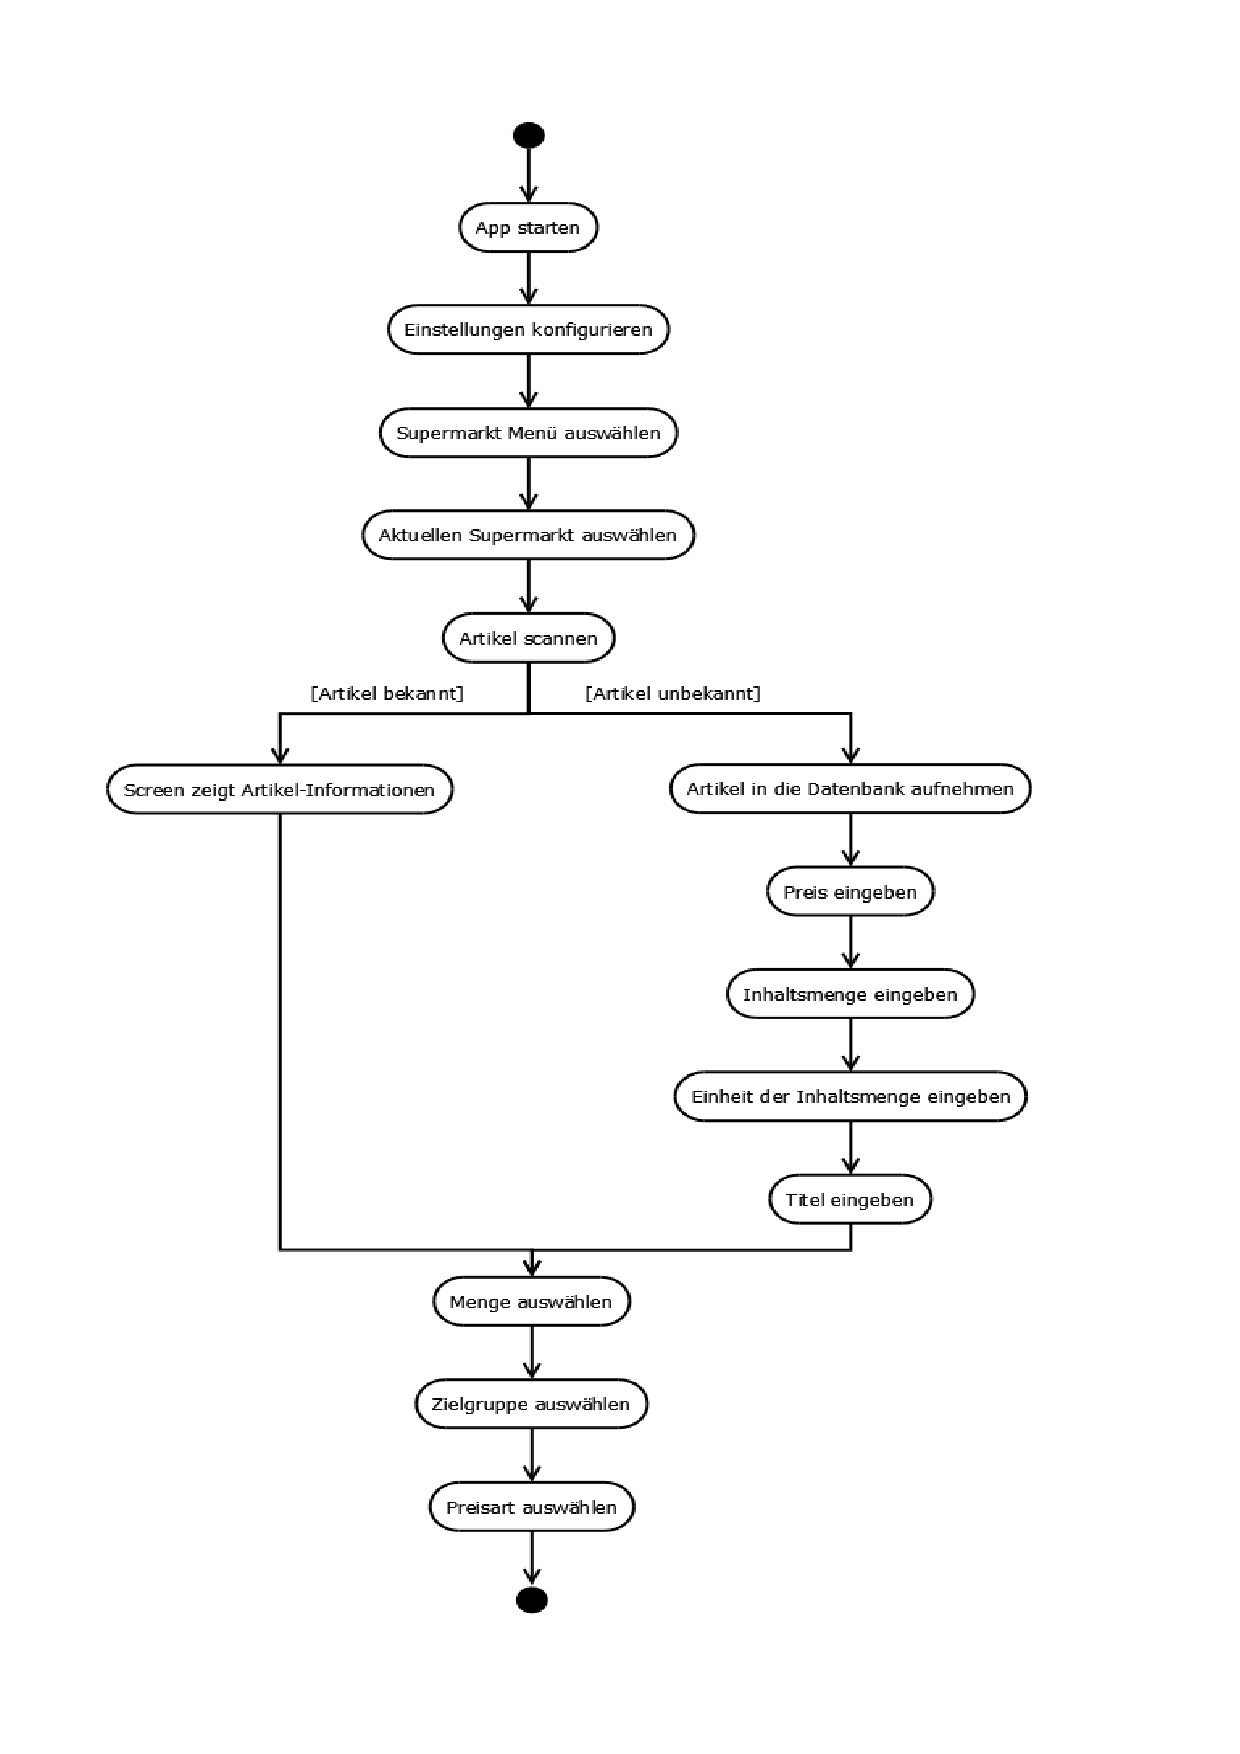
\includegraphics[trim = 17mm 0mm 0mm 20mm,clip, scale=0.7]{Aktiv-Einkauf.pdf}
\\
\footnotesize Abbildung 6: Aktivitätsdiagramm-Einkauf
\normalsize
\subsubsection*{Entwicklung}
%TO DO - TE: einpflegen
\newpage
\subsection{Nutzerverwaltung}
Die Nutzerverwaltung ermöglicht dem Nutzer die individuelle Zuweisung von anderen Accounts als Gruppenmitglieder zu bereits erstellten Gruppe. Ziel dessen ist die vereinfachte Finanzverwaltung wärend des Einkaufes, sowie die Möglichkeit komplexere Auswertung durchzuführen.

\subsubsection*{Design}
\hspace*{-10mm} 
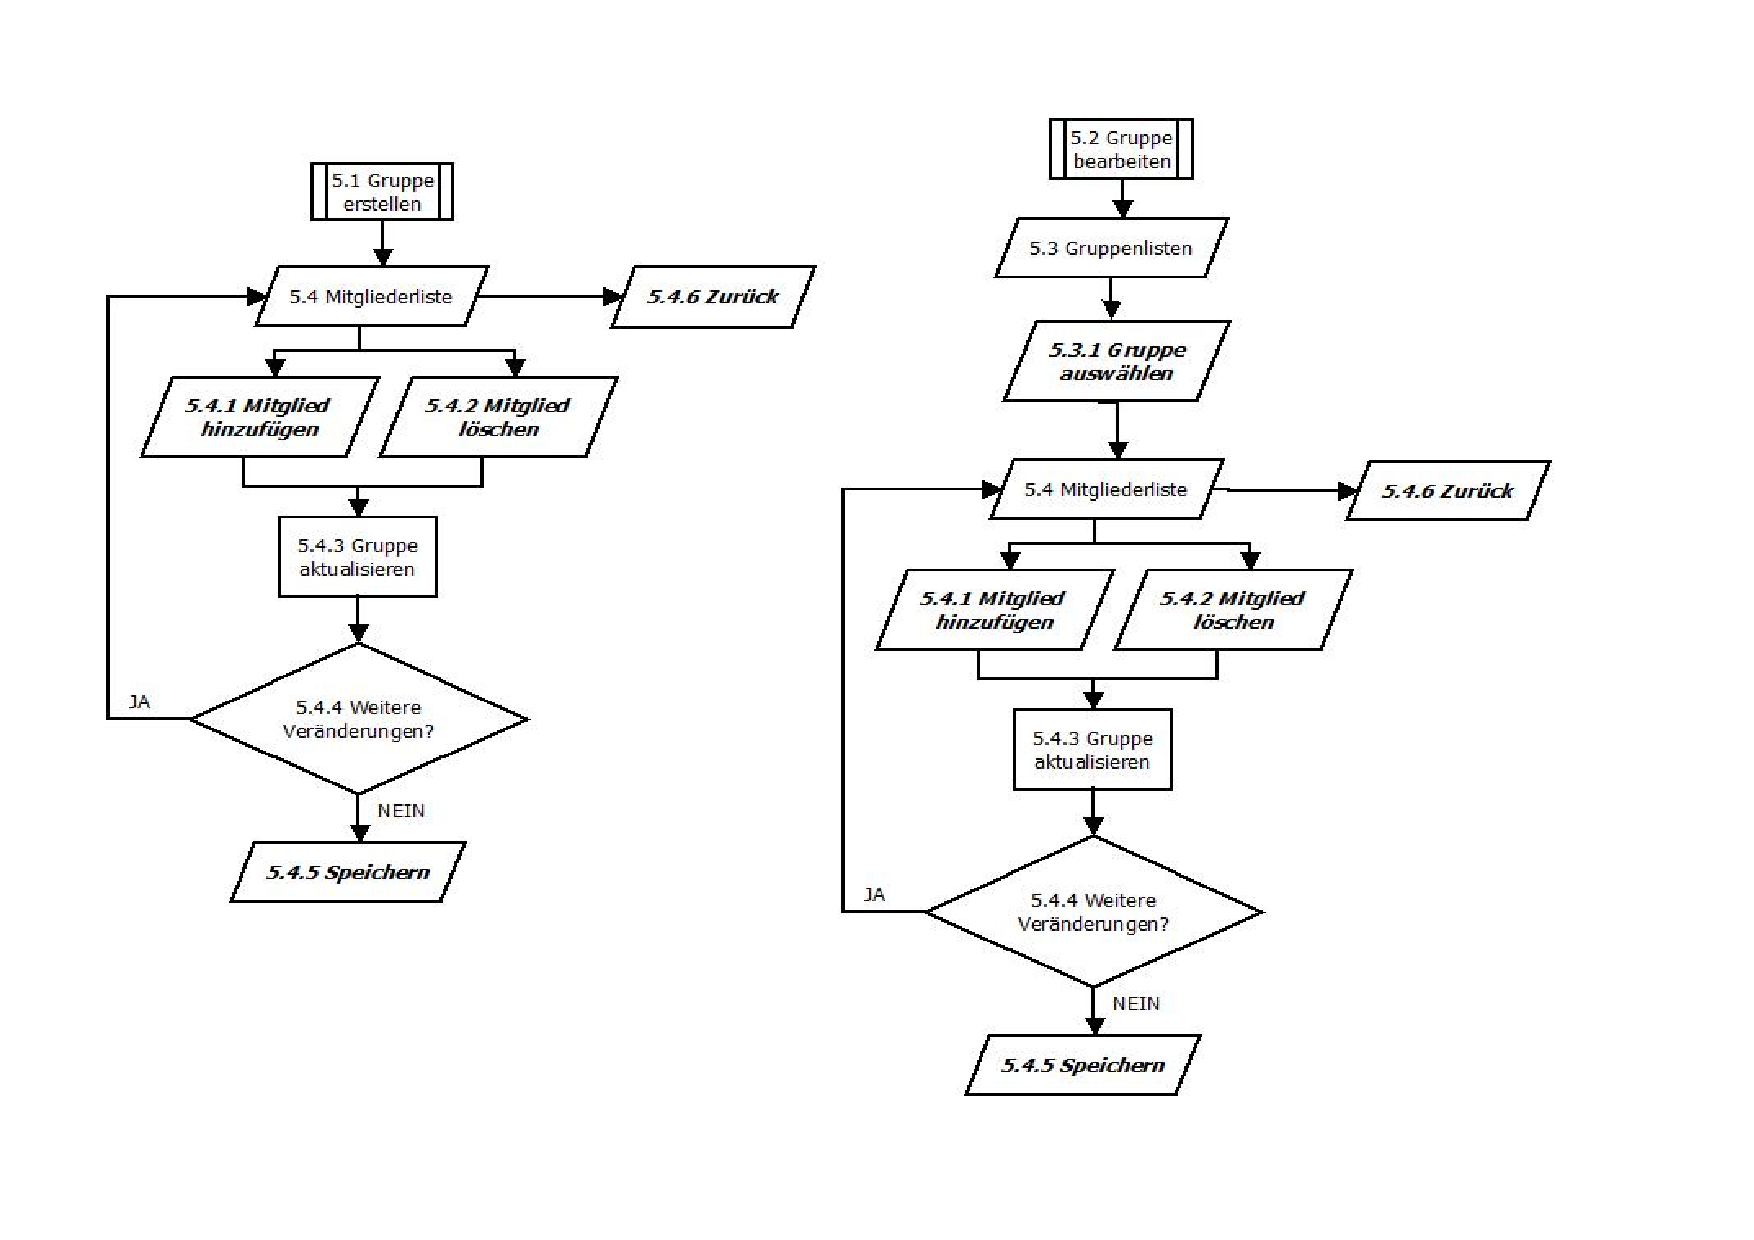
\includegraphics[trim=10mm 20mm 0mm 20mm,clip, scale=0.7]{Gruppenverwaltung.pdf}
\\
\footnotesize Abbildung 7: Gruppenverwaltung
\normalsize
\newline
\newline
Die Gruppenverwaltung wird in zwei Teile unterteilt. Der Erste beschreibt die Gruppenerstellung. Wie im Flussdiagramm zu sehen, kann eine Gruppe angelegt werden, indem zunächst der Nutzer die Menüoption Mitgliederliste wählt und hier eine Gruppe erstellt. Dabei können Mitglieder hinzugefügt bzw. auch gelöscht werden.
\subsubsection*{Entwicklung}
Die Entwicklung hat lediglich den Teil der eigentlichen Gruppenerstellung integriert. Der Nutzer legt einen Gruppennamen fest und kann daraufhin die registrierten Nutzer hinzufügen und ggf. wieder entfernen. Ist die Gruppe erstellt, kann gespeichert werden.
Diese kann im Nachhinein noch nicht geändert werden, weil die Gruppe nicht angezeigt wird. Dies ist ein Problem, welches die Entwickler noch ausbessern werden.
\newpage
\subsection{Auswertung}
Der Nutzer hat die Möglichkeit vergangene Einkäufe auswerten zu lassen. Es gibt die zeitliche Eingrenzung und eine Gruppenmitgliedereingrenzung, bei der alle vergangenen Einkäufe von bestimmten Gruppen zusammengefasst werden.
\\
\\
\hspace*{-10mm} 
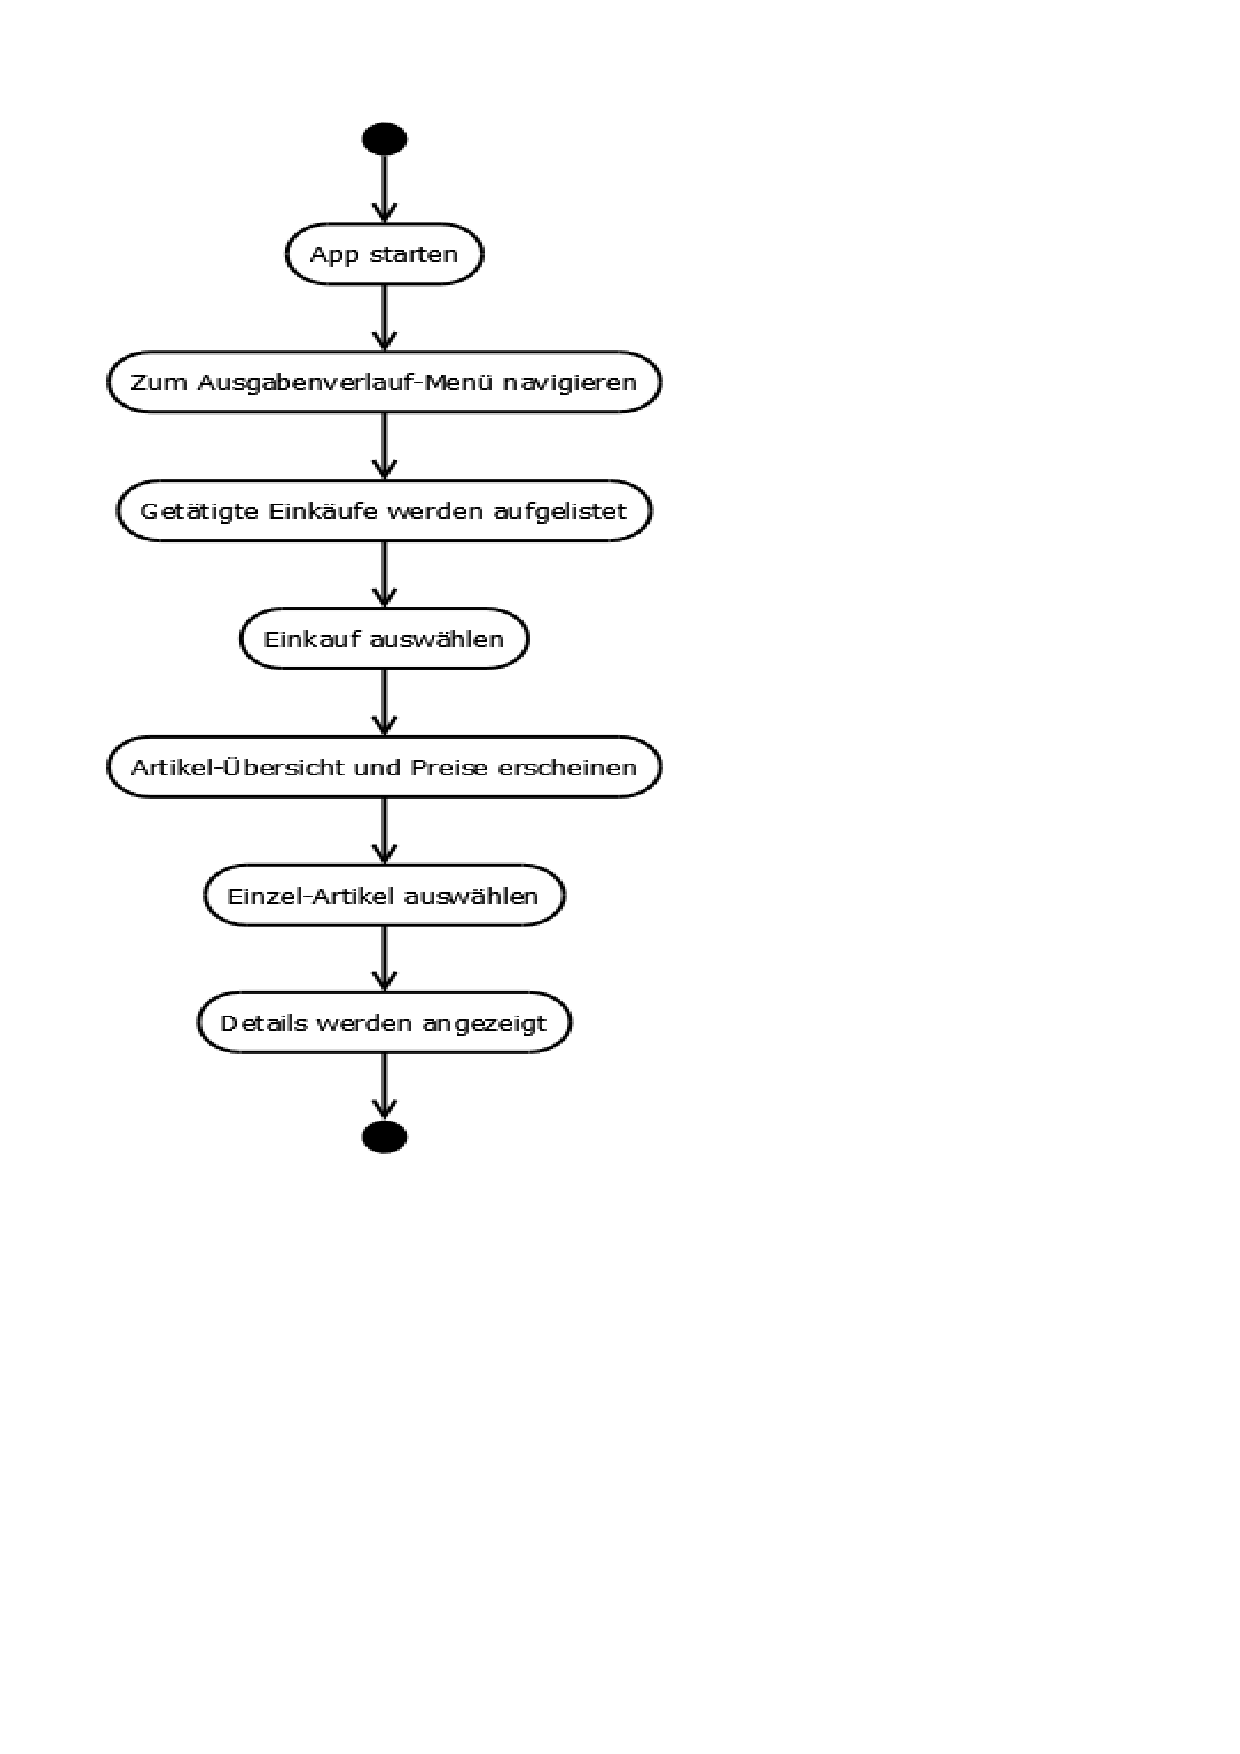
\includegraphics[trim = 17mm 130mm 0mm 20mm, clip, scale=0.9]{Aktiv-Ausgabe.pdf}
\\
\\
\footnotesize Abbildung 8: Aktivitätsdiagramm-Ausgabenverlauf
\normalsize
\\
\newpage
\subsubsection*{Zustandsdiagramm}
 „Ausgabenverlauf anzeigen“
\\
\\
\hspace*{-10mm} 
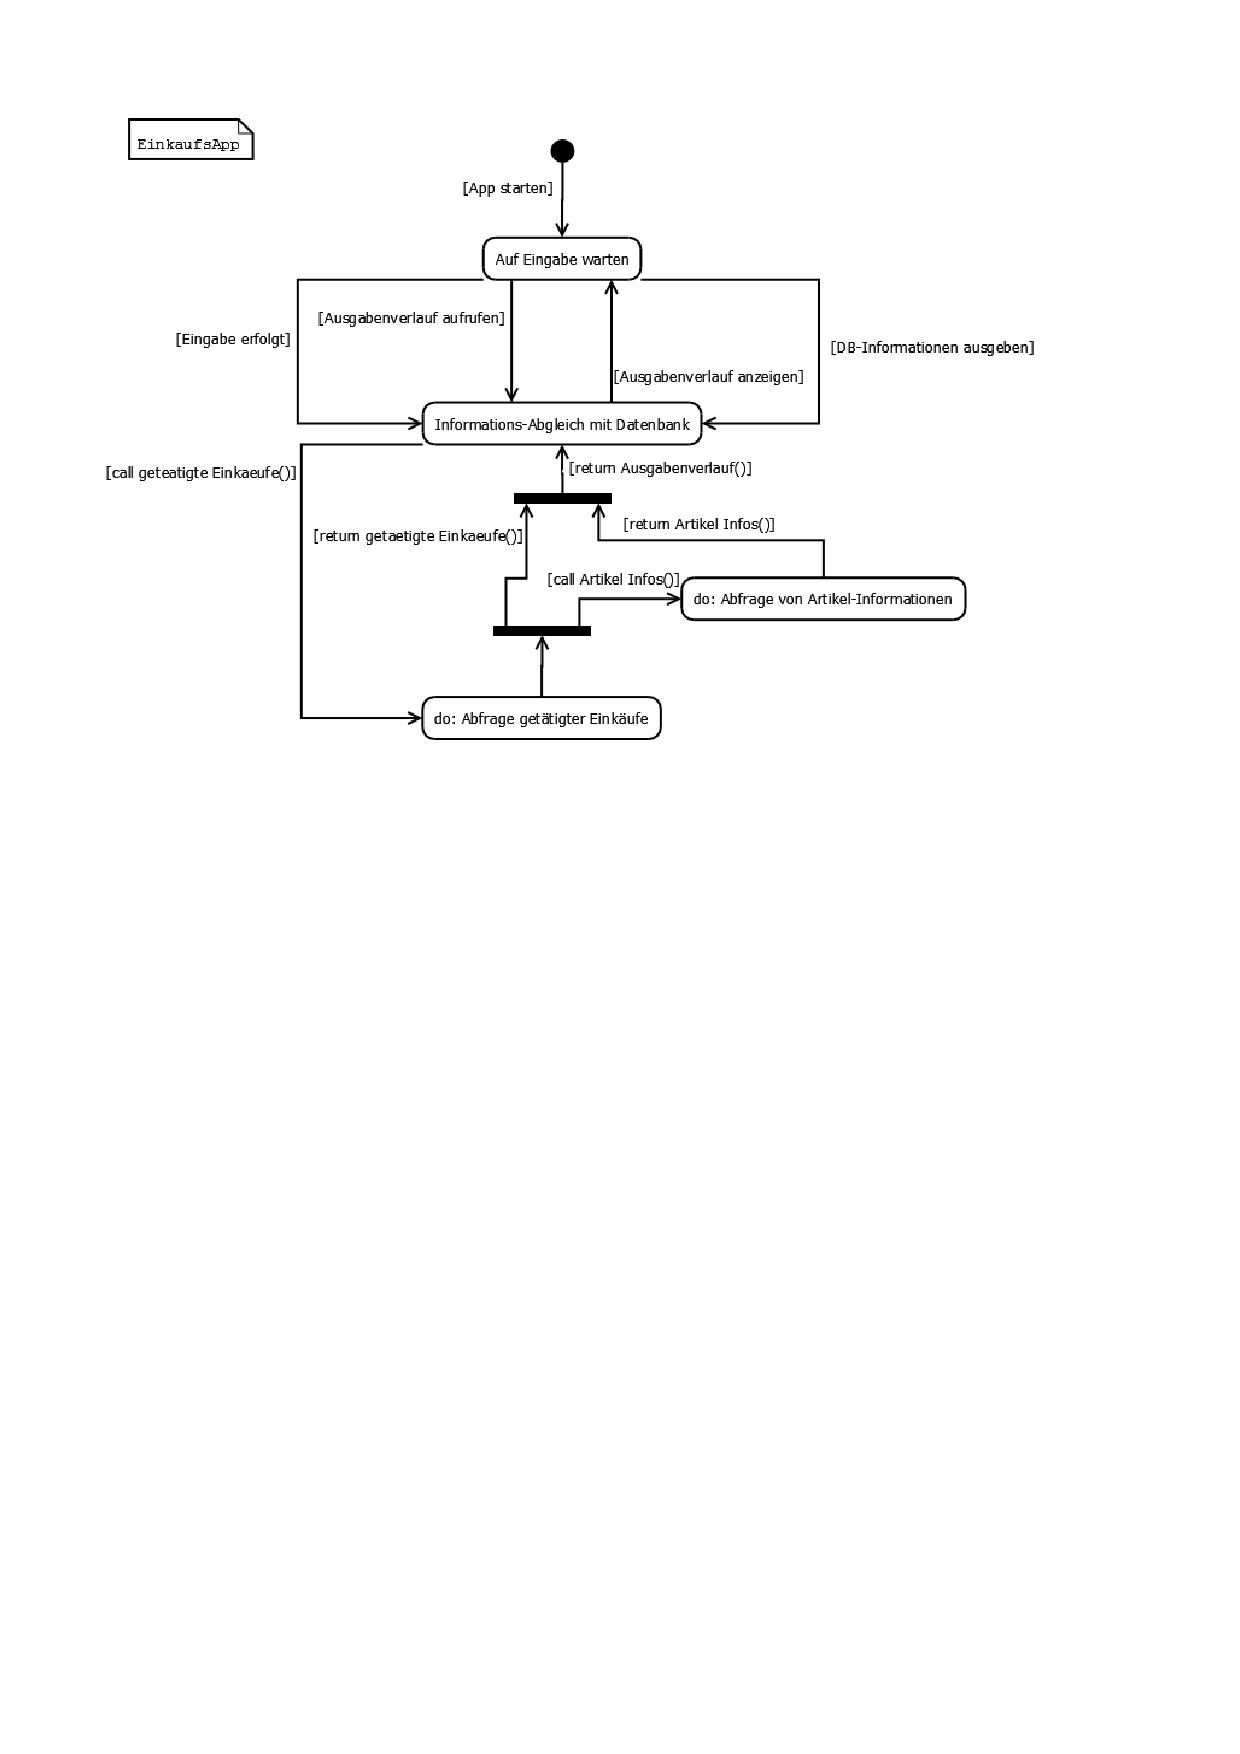
\includegraphics[trim = 17mm 130mm 0mm 20mm,clip]{Zustand.pdf}
\footnotesize Abbildung 9: Zustandsdiagramm
\normalsize
\subsubsection*{Design}
\hspace*{-10mm} 
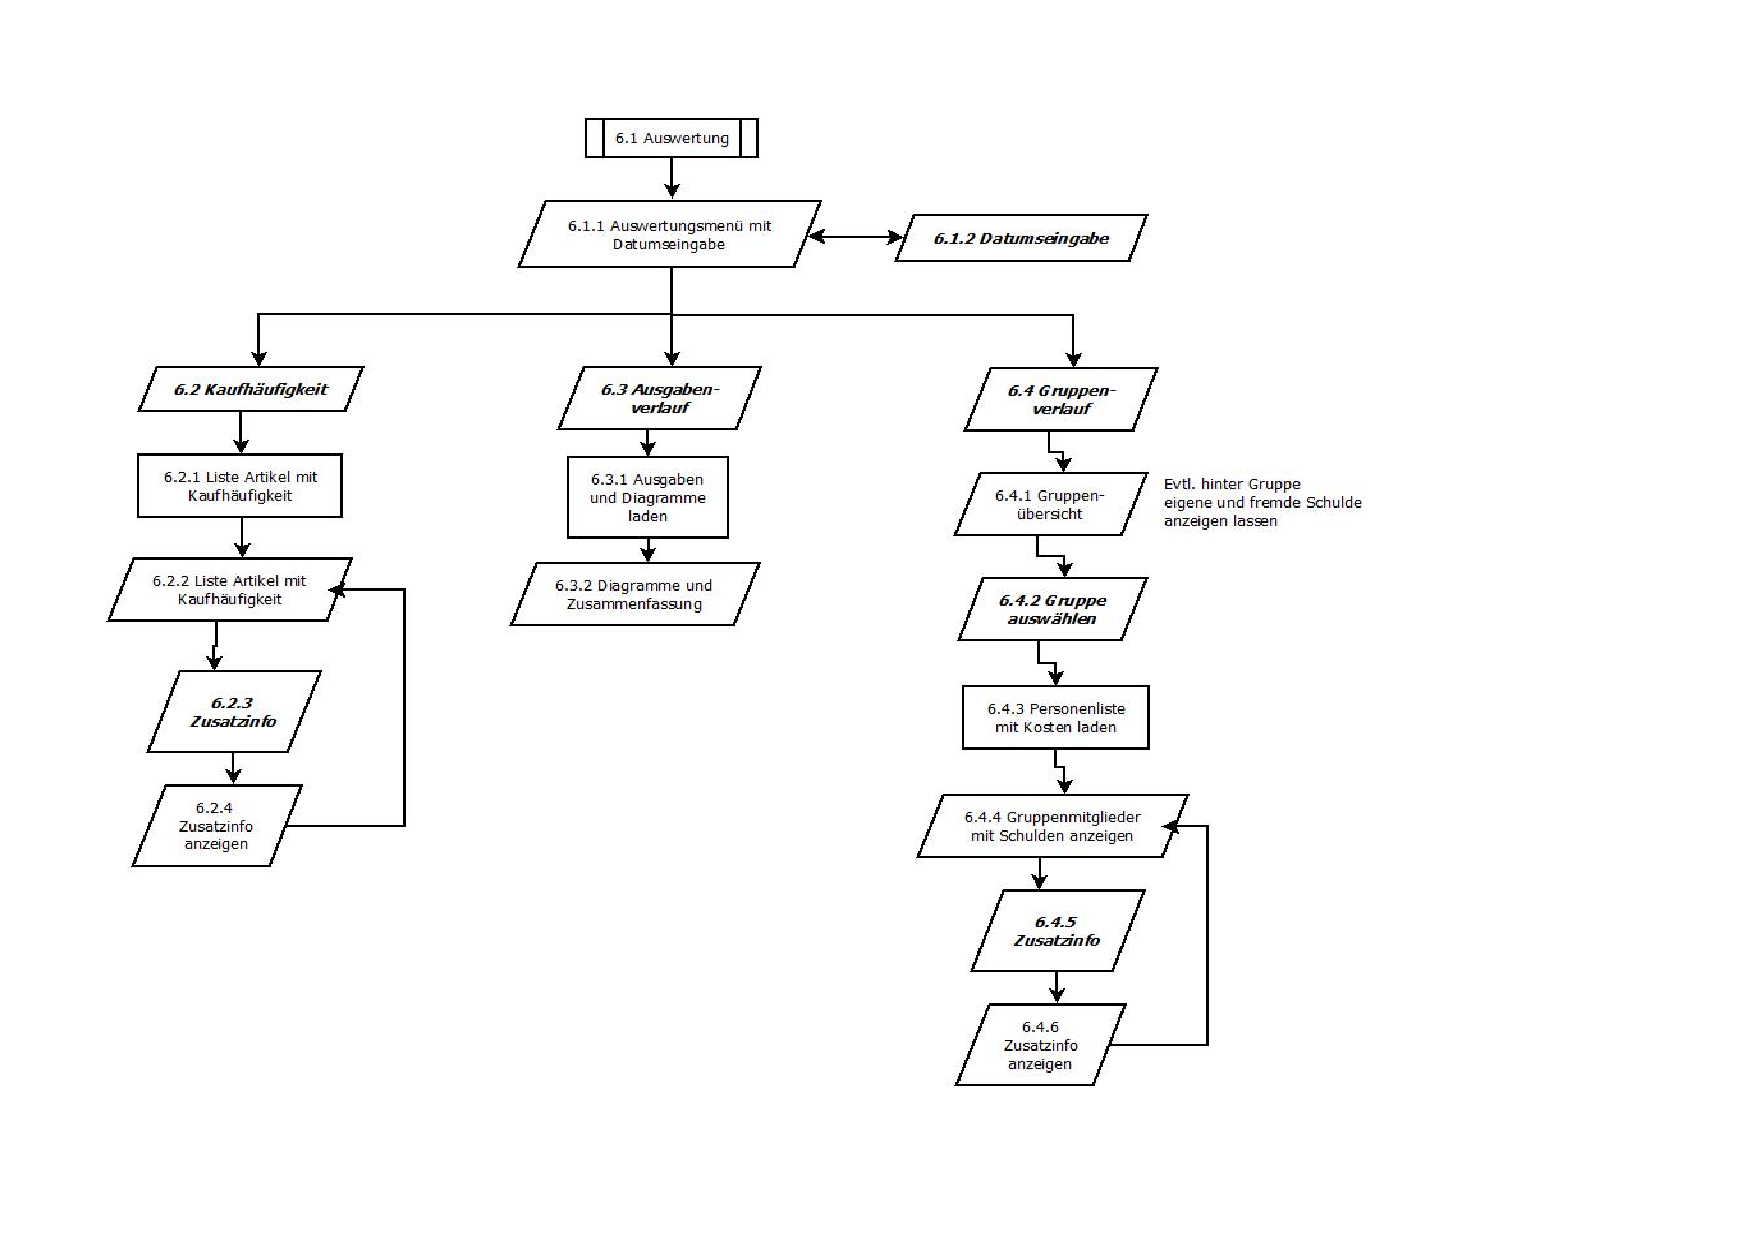
\includegraphics[trim = 20mm 60mm 0mm 20mm,clip,scale=0.8]{Auswertung.pdf}
\footnotesize Abbildung 10: Auswertung
\normalsize
\\
\subsubsection*{Entwicklung}
%MH: Update von Eric einholen
%TO DO - HD: Eric nochmal anschreiben, wie es jetzt genau stant ist
%HD - 22.12.2015 Ja es wurde was umgesetzt. Ich weiß nur nicht, wie ich hierzu eine Text formulieren soll, der nicht wie Handbuch klingt
Wie im Programmablaufplan beschrieben, gibt es im View „Auswertung“ die drei Optionen Kaufhäufigkeit, Ausgabenverlauf und Gruppenverlauf. In jedem dieser Optionen muss ein Start- und Enddatum vom Nutzer festgelegt werden. Je nachdem welche Option ausgewählt wurde, sind die vom System gebende Informationen unterschiedlich. Da es aber weiterhin noch Probleme mit dem Einkaufsprozess gibt, kann die Auswertungsfunktion noch nicht genutzt werden.
%HD- Optionen werden am 24.12.15 eingefügt
\newpage
\section{Problemzusammenfassung}
%Hier wird das Ergebnis beschrieben.
\subsection{Usability der App}
Zusammengefasst kann die Version 1.0 der EinkaufsApp Nutzer registrieren und anmelden, sowie den Einkaufsprozess durchführen. Außerdem können Gruppen erstellt und verwaltet werden. Der Auswertungsprozess wurde in Anbetracht der Zeit nicht umgesetzt. Hinsichtlich des Optik wurde kein Corporate Design - Corporate Identity entwikelt, um die Benutzerfreundlichkeit dennoch zu gewährleisten, implementierten die Entwickler ein schlichtes Interface im aktuellen Web Stil.
\newpage
\subsection{Organisation und Projektmanagement}
%MH: der Inhalt beist sich etwas mit der überschrift - lasst uns noch was besseres finden
Allem voran muss erwähnt werden, dass dieses Projekt enorm zeitkritisch war und daher die Planungsphase nahe zu vollständig übersprungen werden musste. Ebenfalls sind Design und Implementation stark parallelisiert abgelaufen. Um innerhalb von zwei Monaten ein lauffähiges und qualitätsgesichertes Software-Produkt zu erstellen, bedarf es eines überschaubaren und für alle Mitglieder transparenten Projektes, aber allem voran auch ein, gezielt auf die Herausforderungen, zugeschnittenes Team, welches die benötigten Skills und das Know How bereits mitbringt. Ebenfalls ist es sehr wertvoll, wenn die Beteiligten bereits zuvor zusammen gearbeitet haben und untereinander mit Tools und Konventionen vertraut sind, oder zumindest in der Lage sind unter formalen Bedingungen zu arbeiten. Da naturgemäß in unserem Umfeld diese Voraussetzungen nur zu sehr geringen Teilen erfüllt werden können, ist auch ein sehr kritischer Projektablauf unausweichlich. Um diesen Schwierigkeiten entgegen zu wirken, wäre eine klarer Abgrenzung von Aufgabenbereichen
und Skills und auch das Vertrauen in diese Entscheidungen notwendig gewesen. Unglücklicherweise fehlte auch hier wieder die bereits erwähnte Planungsphase, die aber auch aus Zeit- und Lokalitätsgründen nicht umsetzbar war. Im weiteren Verlauf wurde dann eine zusätzliche Organisationseinheit zwischen dem Gesamtprojekt und den einzelnen Entwicklern eingefügt, um einen besseren Überblick zu gewährleisten und schneller Entscheidungen treffen zu können. An dieser Stelle lässt sich auch die obligatorische Diffizilität, die aus den unterschiedlichen Engagements entsteht erwähnen. Nach den vorangegangenen Ausführungen zu den kritischen Komponenten des Projektes sollte selbstredend sein, dass es ohne überdurchschnittlichen Einsatz jedes einzelnen Beteiligten
unmöglich zu 100\% in gegebener Zeit mit derartig begrenzten Ressourcen abgeschlossen werden kann. Nun sind naturgemäß die intrinsischen Beweggründe, sowie die Möglichkeiten der einzelnen Personen verschieden. Somit verbleibt die Aufgabe aller Beteiligten im Rahmen der gegebenen
Bedingungen das bestmöglich Ergebnis zu erzielen.
\newpage
\section{Projektabschluss}
\subsection{Fertiges Produkt}
\subsection{Aussichten}
nicht umgesetzte Ideen --> siehe Excelliste
\newpage
\section{Lesson learned}
%TO DO - MH (fazit)
\newpage
\section*{Quellen}
\addcontentsline{toc}{section}{Quellen}
\subsection*{Internetquellen}
\begin{itemize}
\item[1.]Ionic Framework: \url{http://ionicframework.com/}
\item[2.]Ionic Guide: \url{http://ionicframework.com/docs/guide/}
\item[3.]Ionic Getting Started: \url{http://ionicframework.com/getting-started/}
\item[4.]ngCordova - Plugin Seite \url{http://ngcordova.com/}
\item[5.]BarCode Scanner : Plugin \url{hhttp://ngcordova.com/docs/plugins/barcodeScanner/}
\item[6.]Beispiel Projekt: \url{https://github.com/bastisk/suedm}
\item[7.]Editor: \url{http://brackets.io/}
\item[8.]Angular JS-Kurs: \url{https://www.codeschool.com/courses/shaping-up-with-angular-js/}
\item[9.]Tutorial zum Routing: \url{https://scotch.io/tutorials/angular-routing-using-ui-router}
\item[10.]App-Projekt: \url{http://www.mobile2b.de/ablauf-app-projekt/}
\item[11.] Dokumentationshilfe: \url{http://www.tellsbells.de/dokuwebsite/tbdokumentation.pdf}
\item[12.] Dokumentationshilfe: \url{https://www.lecturio.de/magazin/projekte-dokumentieren/}
\item[13.] Open Source mit API über eine einfachen HTTP-GET-Reguest: \url{http://www.opengtindb.org/api.php}
\item[14.] Suchmaschine der Firma die GTIN-Nummern verwaltet: \url{http://www.gepir.de/v31/V31_client/gtin.aspx}
\end{itemize}
\newpage
\section*{Organisationstools}
\begin{itemize}
\item[-]Zentrale Ablage: GitHub
\item[-]Diskussionsrunden: Slack
\item[-]Informationsaustausch: via Email
\item[-]Diagramme darstellen: via Dia 
\item[-]Kreieren von Web-Prototypen: proto.io
\item[-]Datenbanken und Datenbankenverwaltung: MongoDB, RoboMongo
\end{itemize}
\newpage
\section*{Anhang}
\addcontentsline{toc}{section}{Anhang}
\begin{itemize}
\item Anhang [1]: Pflichtenheft
\item Anhang [2]: Handbuch
\item Anhang [3]: Installationsanleitung
\item Anhang [4]: EER-Diagramm
\item Anhang [5]: Proto.io Design
\item Anhang [6]: Prototyp
\item Anhang [7]: MVP
\item Anhang [8]: Main PAP
\item Anhang [9]: Datenfluss
%HD: Ich weiß nicht,ob wir von den Designern alle Datenflüsse anhängen sollen
%MH: warum nicht?
\item Anhang [10]: ER Modell 
\item Anhang [11]: MongoDB-Klassendiagramm
%HD: Da im Development Repository das MongoDB_v2 ggf.
%MH: da liegt jetzt auch ein v3 drinne -> das ruig nehmen
\item Anhang [12]: Factories

%HD: ich hoffe, dass ich nichts vergessen habe


\end{itemize}
\end{document}

    Status API Training Shop Blog About Pricing 

    © 2015 GitHub, Inc. Terms Privacy Security Contact Help 

    Status API Training Shop Blog About Pricing 

    © 2015 GitHub, Inc. Terms Privacy Security Contact Help 

